\documentclass[10pt,a4paper]{amsart}
\usepackage[utf8]{inputenc}
\usepackage{amsmath}
\usepackage{amsfonts}
\usepackage{amssymb}
\usepackage{amsthm}
\usepackage{hyperref}
\usepackage{mathrsfs}
\usepackage{listings}
\usepackage{ textcomp }
\usepackage{hyperref}
\usepackage{tikz-cd}
\usepackage{verbatim}
\usepackage{enumerate}
\usepackage{cite}
\usepackage{multirow}
\theoremstyle{definition}
\newtheorem{definition}{Definition}
\numberwithin{definition}{section}
\newtheorem{example}[definition]{Example}
\newtheorem{remark}[definition]{Remark}
\newtheorem{claim}[definition]{Claim}
\newtheorem{corollary}[definition]{Corollary}
\newtheorem{question}[definition]{Question}
\newtheorem{theorem}[definition]{Theorem}
\newtheorem{proposition}[definition]{Proposition}
\newcommand{\Mod}[1]{(\mathrm{mod}\ #1)}
\renewcommand\qedsymbol{$\blacksquare$}
\author{James Marshall Reber}
\address{Department of Mathematics, Purdue University, West Lafayette, IN 47907}
\email{marsha71@purdue.edu}
\title{Mixing Times of Random Walks on Various Combinatorial Objects}
\date{July 2018}
\thanks{The author would like to thank Graham White, Indiana University and the NSF for the opportunity to work on this project.   }
\begin{document}

\begin{abstract}
   A classic mixing time result, due to Bayer and Diaconis, is on how many riffle shuffles are required to shuffle a deck of n cards - the required number is $\frac{3}{2} \log_2(n)$. In this paper, we explore the mixing times of random walks on various graphs using a combinatorial method called coupling. In particular, we give upper bounds on the mixing times of certain kinds of random walks on diagonal gluings of $2$-regular graphs, repeated gluings of copies of the complete graph of size three, certain families of $3$-regular graphs, and conjecture some possible generalizations.
\end{abstract}
\maketitle


\tableofcontents

\section{Introduction} \label{sec:intro} 
When describing the mixing time of random walks, we are really discussing what it means to be ``sufficiently close to random'' after a certain amount of time, or rather how long would we need to run a Markov chain until it is within $\epsilon > 0$ of its stationary distribution. The prototypical example of this comes from shuffling a deck. When shuffling a deck, we would like to guarantee that we have a fair deck, or one in which all possible ordering of cards are possible. The mixing times of various shuffles, such as the random transposition shuffle, the riffle shuffle, and top-to-random shuffle, have all been studied and have tight bounds on their mixing times \cite{aldous1986shuffling}. Mixing times can, however, be studied in contexts other than card shufflings; for example, one can ask how long it takes a random walker on a graph to be ``sufficiently random'' among all possible states on the graph.

Throughout this paper, we are concerned with finding the mixing times of random walks on some special classes of graphs. In Section \ref{subsec:mct} and \ref{subsec:gt}, we outline some of the necessary theory and notation from Markov chains and graph theory. In Section \ref{sec:two}, we will explore the mixing times of random walks on $2$-regular graphs glued diagonally (see Figures \ref{fig:graph1} and \ref{fig:graph2} respectively). In Section \ref{sec:three}, we will explore the mixing times of random walks on a graph formed by gluing copies of triangles (or the complete graph on three vertices) on each vertex of degree two repeated $k$ times (see Figure \ref{fig:graph4}), as well as discuss a result on the mixing time of a random walk on the complete graph glued repeatedly along a single vertex (see Figures \ref{fig:graph3} and \ref{fig:graph16}). Finally, in Section \ref{sec:four}, we will explore mixing times of a random walk on the prism graph, M\"{o}bius ladder graph, and the generalized Petersen graph $\text{GP}(n,k)$ (see Figures \ref{fig:graph9}, \ref{fig:graph11}, and \ref{fig:graph13} respectively) as well as their triangulated versions (see Figure \ref{fig:graph8}), and finish by giving some possible directions for future research. 

\subsection{Markov Chain Theory}\label{subsec:mct}

We first introduce some basic concepts on Markov chains. We will be working with a discrete probability space throughout. 
\begin{definition}
We call a sequence of random variables $\{X_i\}_{i = 0}^{\infty}$ on a common state space $\Omega$ a \textbf{Markov chain} if it satisfies the \textbf{Markov property}; that is, for a probability measure $\mathbf{P}$ on $\Omega$, we have 
\[ \mathbf{P}\{X_n = y \ | \ X_0 = x_0, \ldots,X_{n-1}= x_{n-1}\} = \mathbf{P}\{X_n = y \ | \ X_{n-1} = x_{n-1}\}. \]
\end{definition}
\noindent Informally, this means that the probability of a future event happening depends only on the information of the current event. Put into the context of a random walker, if the $\{X_i\}_{i=0}^{\infty}$ are random variables denoting the location of the random walker, then the Markov property states that the probability of where the walker will go in the next step depends only on where the walker is now, and not how the walker got there. 

\begin{remark}
Sometimes the indices will be dropped when referring to Markov chains, e.g. we will write $\{X_i\}$ instead of $\{X_i\}_{i=0}^{\infty}$. 
\end{remark}

\begin{definition}
We define a transition matrix to be a matrix $P$ such that 
\[ P(x,y) = \mathbf{P} \{X_n = y \ | \ X_{n-1} = x_{n-1}\}, \]    
where $X_i \in \{X_i\}_{i=0}^{\infty}$. 
\end{definition}

\begin{proposition}
We have that $P^t(x,y)$, $t > 0$, is the probability of going from state $x$ to state $y$ in $t$ steps.
\end{proposition}

\begin{proof}
We give a sketch of the proof here, proceeding by induction. Notice that it holds for $t = 1$ by definition. We will show the case $t=2$ for clarity. In this case, we have the probability of going from a state $x$ to a state $y$ in two steps is the same as going from a state $x$ to any intermediate state $z \in \Omega$ in one step, and then from state $z$ to state $y$. Since it could be any intermediate state, we take a union over these probabilities; that is,
\[ \{X_2 = y \ | \ X_0 = x\} = \bigcup_{z \in \Omega} \{X_{1} = z \ | \ X_{0} = x\} \cap \{X_{2} = y \ | \ X_{1} = z\}. \]
Notice that $\{X_1 = z \ | \ X_0 = x\}$ is independent of $\{X_2 = y \ | \ X_1 = z\}$ under our probability measure. We apply our probability measure to both sides to get 
\[ \mathbf{P} \{X_2 = y \ | \ X_0 = x \} = \sum_{z \in \Omega} \mathbf{P} \{X_{1} = z \ | \ X_0 = x\} \mathbf{P} \{X_2 = y \ | \ X_1 = z\}.\]
However, we can use our transition matrix notation; rewriting the right hand side, we have
\[ \mathbf{P} \{X_2 = y \ | \ X_0 =x \} = \sum_{z \in \Omega} P(x,z)P(z,y) = P^2(x,y) \]
by matrix multiplication, as desired. Now, assume the statement holds for $d > 0$. That is, 
\[ \mathbf{P} \{X_d = y \ | \ X_0 = x\} = P^d(x,y).\]
We want to then show the statement holds for $d+1$. However, this is analogous to the arugment for $t=2$, and so we end up with
\[ \mathbf{P} \{X_{d+1} = y \ | \ X_0 = x \} = \sum_{z \in \Omega} \mathbf{P} \{X_{d+1} = y, X_d = z \ | \ X_0 = x\}\]
\[ = \sum_{z \in \Omega} P^d(x,z)P(z,y) = P^{d+1}(x,y).\]
\end{proof}

\begin{remark}
Since we have that $P^t(x,y)$ is the probability of going from $x$ to $y$ in $t$ steps, this shows that the transition matrix encodes all of the information of the Markov chain.
\end{remark}

\begin{remark}
Throughout, we take $\Omega$ to be the state space for our Markov chain and $P$ to be its transition matrix unless stated otherwise.
\end{remark}

\begin{definition}
We say that a Markov chain is \textbf{irreducible} if for all $x, y \in \Omega$ we have some $0 \leq r < \infty$ such that $P^r(x,y) < \infty$. 
\end{definition}
\noindent In other words, it is irreducible if it is possible for the Markov chain to reach every state from every state in a finite number of steps. 
\begin{definition}
We define the \textbf{period} of a state $x \in \Omega$ to be 
\[ \mathscr{T}(x) := \gcd \{t \geq 1 \ | \ P^t(x,x) > 0  \}. \]
\end{definition}
\noindent In other words, the period is the greatest common divisor of the set of times where $x$ has a non-trivial probability of returning to $x$. 
\begin{definition}
We say that a chain is \textbf{aperiodic} if $\mathscr{T}(x) = 1$ for all $x \in \Omega$, and we say the chain is \textbf{periodic} otherwise. 
\end{definition}
\begin{definition}
We say that a distribution, which will be a row vector, $\pi$ on $\Omega$ is a \textbf{stationary distribution} if it satisfies 
\[ \pi P = \pi. \]
\end{definition}
\begin{definition}
We say $\hat{\pi}$ is a \textbf{limiting distribution} if it is a distribution on $\Omega$ and 
\[ \lim_{t \rightarrow \infty} P^t(x,y) = \hat{\pi}(y). \]
\end{definition}
The reason we care about periodicity and irreducibility is due to the following theorem.

\begin{theorem}\label{thm:1}
If a Markov chain is irreducible and aperiodic, then it has a unique stationary distribution which is also its limiting distribution.
\end{theorem}

\begin{proof}
This follows from Corollary 1.17 and Theorem 4.9 in \cite{LevinPeresWilmer2006}.
\end{proof}

While the proof of the above theorem is involved, we give some intuition as to why you need these conditions. If your Markov chain was not irreducible, then that means there are two separate components. As a result, if there even is a stationary distribution, it will not be unique in any sense as there will be a stationary distribution for each irreducible component. Aperiodicity is important as it ensures that our stationary distribution is the limiting distribution. Imagine the Markov chain on the cycle $\mathbb{Z}/4\mathbb{Z}$ which moves left with probability $1/2$ and right with probability $1/2$. We see that there is no limiting distribution, as its distribution relies on whether or not its on an even or odd number. Thus, we really do need both conditions for this to hold.

Throughout, we will assume all of our Markov chains will be aperiodic and irreducible so that they will have unique stationary distributions that also are their limiting distributions. The stationary distribution will really be how we measure ``sufficiently random.'' Taking our Markov chain to be aperiodic and irreducible, we have that in the long run it will be close to this stationary distribution. Referring back to the shuffling example, our stationary distribution is the uniform distribution on all possible configurations of the deck, and so being close to the stationary distribution means being close to having a fair deck.

We now need to formalize the notion of distance between two distributions. We define the \textbf{total variation distance} between probability distributions $\mu$ and $\nu$ on $\Omega$ to be 
\[ || \mu - \nu ||_{TV} = \max_{A \subseteq \Omega} |\mu(A) - \nu(A)|.\]

\begin{remark}
We can equivalently define total variation distance to be 
\[ ||\mu - \nu ||_{TV} = \frac{1}{2} \sum_{x \in \Omega} \big|\mu(x) - \nu(x)\big| = \sum_{\substack{x \in \Omega \\ \mu(x) \geq \nu(x)}} \big(\mu(x) - \nu(x)\big).\]
The proof of the equivalence follows from Proposition 4.2 in \cite{LevinPeresWilmer2006}. A good visualization of total variation distance can be seen in Figure 4.1 in \cite{LevinPeresWilmer2006}.
\end{remark}

\begin{remark}
It can be shown that total variation distance is a metric, and so really does satisfy the intuition of distance. With the above equivalence, we also see that it is closely related to the $L^1$ norm.
\end{remark}

In particular, we would like to study the position of a random walker in comparison to its stationary distribution. As a result, we define
\[ d(t) := \max_{x \in \Omega} ||P^t(x, \cdot) - \pi ||_{TV}\]
to be the distance between $P^t(x, \cdot)$, the random walker which is starting at $x$ whose position is $\cdot$ at time $t$, and $\pi$. Referring back to the example of shuffling decks, this tells us how close our deck, starting at configuration $x$, is to stationarity after $t$ shuffles. We would like to know roughly when $P^t$ is close to $\pi$; that is, when their total variation distance is within $\epsilon >0$. This notion makes sense as $d(t)$ is decreasing as $t$ increases. 

\begin{definition}
We define the \textbf{mixing time} to be 
\[ t_{\text{mix}} (\epsilon) := \min \{t \ | \ d(t) \leq \epsilon\}. \]
\end{definition}

Understanding the mixing time of random walks is central to our project, and as a result we would like to be able to get bounds on the mixing time. One method for bounding the mixing time is coupling, which we use throughout. 
\begin{definition}
We define a \textbf{coupling} of two probability distributions $\mu$ and $\nu$ to be a pair of random variables $(X,Y)$ defined on a single probability space $\Omega$ such that 
\[ \sum_{y \in \Omega} \mathbf{P} \{X = x, Y = y\} = \mathbf{P} \{X = x\} = \mu(x) \]
and 
\[ \sum_{x \in \Omega} \mathbf{P} \{X = x, Y = y\} = \mathbf{P} \{Y = y\} = \nu(y).\]
\end{definition}
\noindent That is, a coupling of probability distributions instills a set of rules which determine how the two probability distributions behave relative to one another. However, if we viewed just one probability distribution without the other, we would see that it still satisfies being a probability distribution.

\begin{definition}
We define a \textbf{coupling of Markov chains} with transition matrix $P$ to be a process $(X_t, Y_t)_{t=0}^{\infty}$ with the property that both $\{X_t\}_{t=0}^{\infty}$ and $\{Y_t\}_{t=0}^\infty$ are Markov chains with transition matrix $P$. 
\end{definition}
\noindent For example, think of the random walker starting at location $x$, and the same random walker except starting at location $y$. Then they share a transition matrix, $P$, are both Markov chains, and we can define a set of rules that each walker must adhere to relative to the other.

\begin{definition}
Given a Markov chain on $\Omega$ with transition matrix $P$, we define a \textbf{Markovian coupling} of two $P$-chains to be a \textbf{Markov chain} $\{(X_t, Y_t)\}_{t=0}^{\infty}$ with state sapce $\Omega \times \Omega$ which satisfies, for all $x, y, x', y'$
\[\mathbf{P} \{ X_{t+1} = x' \ | \ X_t =x, Y_t, y\} = P(x,x') \]
\[\mathbf{P} \{ Y_{t+1} = y' \ | \ X_t = x, Y_t = y\} = P(y,y'). \]

In general, we also require that if $X_t = Y_t$ for some $t \geq 0$, then we have $X_s = Y_s$ for all $s \geq t$. That is, once they have coalesced, they stay coalesced. 
\end{definition}

\noindent Markovian couplings are nice in the sense that they are easy to describe. However, Markovian couplings will not always give you the best upper bound. All couplings in this paper will be Markovian.

We now need to connect having information on two random walkers, $P^t(x, \cdot)$ and $P^t(y, \cdot)$, to information on the random walker compared to the stationary distribution.

\begin{proposition}\label{prop:1}
If we define 
\[ \bar{d}(t) := \max_{x,y \in \Omega } ||P^t(x, \cdot) - P^t(y, \cdot)||_{TV},\]
then we have 
\[ d(t) \leq \bar{d}(t).\]
\end{proposition}

\begin{proof}
A proof is given in \cite{LevinPeresWilmer2006}. We will give a sketch here. Since $\pi$ is a stationary distribution, we have 
\[ \pi P = \pi \]
gives us 
\[ \sum_{x \in \Omega} P(x,y) \pi(x) = \pi(y) \]
by matrix multiplication. Furthermore, we have 
\[ \sum_{x \in \Omega} P(x, A) \pi(x) = \pi(A) \]
for any subset $A \subseteq \Omega$. Now, notice that 
\[|P^t(x,A) - \pi(A)| = \left|P^t(x,A) - \sum_{y \in \Omega}P^t(y,A)\pi(y) \right|. \]
Since $\pi$ is a probability distribution, we have
\[\sum_{y \in \Omega} \pi(y) = 1, \]
and so we get
\[ \left|P^t(x,A) - \sum_{y \in \Omega}P^t(y,A)\pi(y)\right| = \left|\sum_{y \in \Omega} \pi(y) \big(P^t(x, A) - P^t(y, A) \big) \right|. \]
By the triangle inequality, this is less than or equal to 
\[ \sum_{y \in \Omega} \pi(y) \big| P^t(x, A) - P^t(y, A) \big|. \]
This is a weighted average, and so in particular we have
\[\sum_{y \in \Omega} \pi(y) \big| P^t(x,A) - P^t(y,A) \big| \leq \max_{y \in \Omega} \big| P^t(x,A) - P^t(y,A) \big| .\] 
This gives us  
\[ d(t) \leq \bar{d}(t).\]
\end{proof}

We see that studying $\bar{d}(t)$ gives us information on $d(t)$, which we can then use to derive the mixing time. We can then use the following theorem to get information on bounding $\bar{d}(t)$, and thus on bounding $d(t)$.

\begin{theorem}\label{thm:2}
For any two Markov chains $\{X_i\}$ and $\{Y_i\}$ over a common state space $\Omega$ with $X_0 = x$, $Y_0 = y$, let $\tau_{\text{couple}}$ be the time of the chains coalesce. That is, 
\[\tau_{\text{couple}} := \min \{t \ | \ X_s = Y_s \text{ for all } s \geq t \}. \]
Then 
\[ d(t) \leq \bar{d}(t) \leq \max_{x,y \in \Omega} \mathbf{P} \{\tau_{\text{couple}} > t \ | \ X_0 = x, Y_0 = y\} \leq \max_{x, y \in \Omega} \frac{\mathbf{E}(\tau \ | \ X_0 = x, Y_0 = y)}{t}.\]
\end{theorem}

\begin{proof}
This a consequence of Corollary 5.5 in \cite{LevinPeresWilmer2006} and Proposition \ref{prop:1}, with the last inequality coming from Markov's inequality.
\end{proof}

We will often want to transform our complicated Markov chain to a much simpler one. We formalize this in the definition below.

\begin{definition}
Let $\{X_t\}$ be a Markov chain. Then the \textbf{quotient Markov chain} $\{X_t'\}$ is the corresponding Markov chain quotiented out by some equivalence relation between states. That is, there's a bijective function between $\{X_t\}$ and $\{X_t'\}$ which preserves transition probabilities. 
\end{definition}

An example of this can be seen in the proof of Proposition \ref{prop:binarylazyrw}. More examples of Markov chains and couplings can be found in the Appendix (Section \ref{appendix}).

\subsection{Graph Theory} \label{subsec:gt}
We now introduce some concepts from graph theory. 
\begin{definition}
We define a \textbf{graph} G = (V,E) to consist of a set of vertices $V$ and a set of edges $E \subseteq V \times V$.
\end{definition}
\noindent In other words, the vertices represent some collection of objects and the edges represent some relation between those objects. We can visually represent graphs by having the vertices be dots and the edges be lines between the dots. 
\begin{remark}
We will be working with \textbf{undirected graphs}, or graphs where if $(x,y) \in E$ then $(y,x) \in E$ as well. A \textbf{directed graph} is a graph such that $(x,y) \in E$ does not imply $(y,x) \in E$. We will also, for the most part, be working with \textbf{simple graphs}, or graphs that do not have any kind of self-loops. Notationally, we have $(x,x) \notin E$ for all $x \in V$.
\end{remark}
\noindent In general, undirected graphs are drawn with just lines as edges (see Figure \ref{fig:graph01}), and directed graphs are drawn with arrows for edges (see Figure \ref{fig:graph0}). 

\begin{remark}
Notice that a Markov chain is a \textbf{weighted digraph}, or a directed graph whose edges have some sort of value, and so we graphically represent Markov chains using directed graphs.
\end{remark}

\begin{figure}
\begin{center}
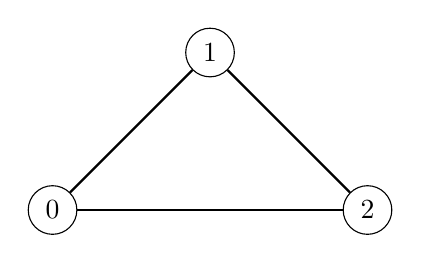
\begin{tikzpicture}
  [main node/.style={circle,draw}]
  \node[main node] (n0) at (10,10) {0};
  \node[main node] (n1) at (12,12) {1};
  \node[main node] (n2) at (14,10) {2};
  
  \path[]
  (n0) [-, thick] edge node [] {} (n1);
  \path[] (n1) [-, thick] edge node [] {} (n2);
  \path[] (n2) [-, thick] edge node [] {} (n0);
\end{tikzpicture}
\end{center}
\caption{The undirected graph with $V = \{0,1,2\}$, $E = \{(0,1), (1,0), (1,2), (2,1), (0,2), (2,0)\}$.}
\label{fig:graph01}
\end{figure}


\begin{figure}

\begin{center}
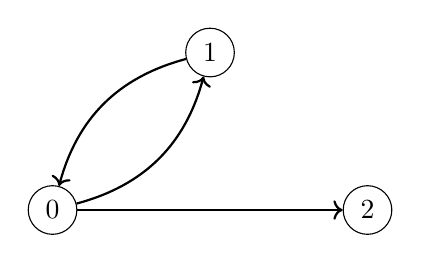
\begin{tikzpicture}
  [main node/.style={circle,draw}]
  \node[main node] (n0) at (10,10) {0};
  \node[main node] (n1) at (12,12) {1};
  \node[main node] (n2) at (14,10) {2};
  
  \path[]
  (n0) [->, bend right, thick] edge node [] {} (n1);
  \path[] (n1) [->, bend right, thick] edge node [] {} (n0);
  \path[] (n0) [->, thick] edge node [] {} (n2);
\end{tikzpicture}
\end{center}
\caption{The directed graph with $V = \{0,1,2\}$, $E = \{(0,1), (1,0), (0,2)\}$.}
\label{fig:graph0}
\end{figure}

\begin{definition}
If $(x,y) \in E$, we say that $x$ and $y$ are \textbf{neighbors}. 
\end{definition}

\begin{definition}
Let 
\[ N(x) := \{y \in \Omega \ : \ (x,y) \in E\} \]
be the set of neighbors for some vertex $x$. Then we say that the \textbf{degree} of $x$ is 
\[ \text{deg}(x) := |N(x)|,\]
or the number of neighbors it has.
\end{definition}

\begin{definition}
Say we have a graph $G$. We define a \textbf{simple random walk} on $G$ to be the Markov chain with state space $\Omega = V$ and transition matrix 
\[ P(x,y) = \begin{cases} \frac{1}{\text{deg}(x)} \ \text{ if } (x,y) \in E \\
0 \ \text{ otherwise.}
\end{cases}\]
\end{definition}
In other words, a random walker will uniformly select a neighbor of the vertex it is at and move accordingly. We note that the simple random walk on $G$ is not always irreducible or aperiodic. If our graph is \textbf{connected}, that is, there exists some path of edges such that $x$ can get to $y$ for all $x,y \in V$, then the simple random walk will be irreducible. To solve the issue of periodicity, we will make our simple random walk \textbf{lazy}. To do so, we simply add a $1/2$ chance to stay in place. 

\begin{definition}
We have a \textbf{lazy random walk} if our transition matrix is then 
\[ P(x,y) = \begin{cases} \frac{1}{2} \ \text{ if } x = y \\ 
\frac{1}{2\text{deg}(x)} \ \text{ if } (x,y) \in E \\
0 \ \text{ otherwise.}\end{cases} \]
\end{definition}

\begin{definition}
We say that a graph is \textbf{s-regular} if $\deg(x) = s$ for all $x \in V$. 
\end{definition}

\begin{definition}
We define the \textbf{complete graph on $n$-vertices} to be the graph where every vertex is connected to every other vertex, and denote it by $K_n$.  
\end{definition}

\begin{definition}
If we have graphs $G_1 = (V_1, E_1)$ and $G_2 = (V_2, E_2)$, then \textbf{gluing} $G_1$ to $G_2$ along vertices $x \in V_1$ and $x' \in V_2$ involves identifying $x$ and $x'$ together, and then attaching all of the edges which are connected to $x$ and $x'$ to this new vertex. 
\end{definition}

\begin{definition}
We define \textbf{triangulating} a graph to be replacing each vertex with a copy of $C(3)$ and appropriately attaching edges to corresponding vertices. More can be seen in Section 4, as well as in Figure \ref{fig:graph8}. 
\end{definition}

\begin{definition}
We define the \textbf{graph metric} $\rho$ to be the function which takes two vertices $v_1, v_2 \in V$ and measures the \textbf{distance} between them; in other words, the minimum number of edges one must take to get from one vertex to another.
\end{definition}

\section{Diagonal Gluings of 2-Regular Graphs} \label{sec:two}

We first define a gluing process on $2$-regular graphs. Start with a $2$-regular graph of size $n$, and identify two vertices $v_1, v_2$ such that $\rho(v_1, v_2) = 2$ to be the corners. At step $k=2$, glue a copy of the $2$-regular graph along one of the corners, and then identify a vertex $v_3$ to be the vertex on the new graph such that $\rho(v_2, v_3) = 2$. Iterate this process for each remaining $k$; that is, identify a vertex to be the corner and glue along that. An example is given in Figure \ref{fig:graph1}. We will use the standard lazy random walk on this graph. In other words, we define the Markov chain on this graph as follows: 
\[ P(x,y) = \begin{cases} \frac{1}{4} \ \ \text{ if } y \in N(x) \text{ and } \text{deg}(x) = 2, \\
\frac{1}{8} \ \ \text{ if } y \in N(x) \text{ and } \text{deg}(x) = 4, \\
\frac{1}{2} \ \ \text{ if } y = x,\\
0 \ \ \text{ otherwise.} 
\end{cases}\]

\noindent Considering even $n$ leads us to the following proposition.

\begin{figure}

\begin{center}
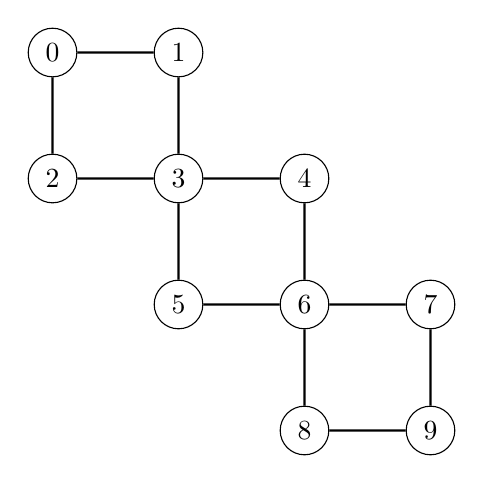
\begin{tikzpicture}
  [scale=.8,auto=left,every node/.style={circle,draw}]
  \node (n0) at (2,17) {0};
  \node (n1) at (4,17)  {1};
  \node (n2) at (2,15)  {2};
  \node (n3) at (4,15) {3};
  \node (n4) at (6,15)  {4};
  \node (n5) at (4,13)  {5};
  \node (n6) at (6,13) {6};
  \node (n7) at (8,13) {7};
  \node (n8) at (6,11) {8};
  \node (n9) at (8,11) {9};
  \foreach \from/\to in {n0/n1, n1/n3, n0/n2, n2/n3, n3/n4, n3/n5, n4/n6, n5/n6, n6/n7, n6/n8, n8/n9, n7/n9}
    \draw [thick] (\from) -- (\to);
\end{tikzpicture}
\end{center}
\caption{Diagonal gluing with $n=4$, $k=3$.}
\label{fig:graph1}
\end{figure}


\begin{proposition}\label{prop:2}
Fix $n$ even and any $k$ for the proposed structure. Let $\{X_i\}$ and $\{Y_i\}$ be two Markov chains with transition matrix $P$ such that they are both lazy random walks on the graph. We have a coupling such that if $\tau$ is the time until they coalesce, then 
\[\max_{x,y \in \Omega} \mathbf{E}(\tau \ | \ X_0 = x, Y_0 = y) \leq \frac{(kn)^2}{2}. \]
In particular, we see   
\[ t_{\text{mix}}(\epsilon) \leq \frac{(kn)^2}{2 \epsilon}\]
\end{proposition}

\begin{proof}
We do a sort of depth-first search approach to our coupling. Let $0$ be the top left most node (i.e. the vertex on the original graph which as at maximal distance from the glued vertex) and define $h : \Omega \rightarrow \{0, \ldots, (kn)/2\}$ to be the function
\[ h(v) = \rho(v, 0). \]
In other words, $h$ measures the relative 'height' of a random walker. Let $X_i$ and $Y_i$ be our random walkers on this graph. We see that the maximum distance will be $(kn)/2$, since the maximal distance on the $2$-regular graph of size $n$ is $n/2$ and we are simply increasing this distance $k$ times. We can divide up our vertices into classes based on their height, and since the vertices in these corresponding height classes will have the same transition probabilities between other height classes, we can push this to a quotient Markov chain. Thus, we can now think of this as a random walk on the chain $\{0, \ldots, (kn)/2\}$ with the transition probabilities 
\[ P(x,y) = \begin{cases} \frac{1}{4} \ \text{ if } y \in N(x) \text{ and } x \neq 0 \text{ nor } \frac{kn}{2}, \\
\frac{1}{2} \ \text{ if } y \in N(x) \text{ and } x = 0 \text{ or } \frac{kn}{2}, \\ 
\frac{1}{2} \ \text{ if } x = y, \\
0 \text{ otherwise.}
\end{cases} \]

Our coupling is now the following: since we can just use the Markov chain given above to model where our walkers are, we couple so that they both move the same direction. If they were to try to move in a direction that doesn't exist at the end points, we just have the walker wait in place. This will preserves the property that $h(X_s) \leq h(Y_s)$, assuming without loss of generality that $X_s$ is closer to $0$. To see how long it takes for the walkers to coalesce, we just need to measure the maximum expected amount of time it takes for a walker to reach $0$. This follows since this is the same as measuring how long it takes $Y_s$ to reach $0$, and since $h(X_s) \leq h(Y_s)$ we get $h(X_s) = h(Y_s) = 0$. Let $\tau'$ be the amount of time it takes a walker $\{X_t\}$ to reach $0$. We set up a series of functions $f_j = \mathbf{E}(\tau' \ | \ X_0 = j)$ such that $f_0 = 0$, 
\[f_j = \frac{1}{4}\left(1 + f_{j-1}\right) + \frac{1}{2}(1+f_j) + \frac{1}{4}(1+f_{j+1})  \]
for $0 < j < (kn)/2$, and 
\[ f_{(kn)/2} = \frac{1}{2}(1+f_{(kn)/2}) + \frac{1}{2}(1+f_{(kn)/2-1}).\]

\begin{claim}\label{claim:1}
For $0 < j < (kn)/2$, 
\[ f_j = 2j + \frac{j}{j+1} f_{j+1}. \]
\end{claim}

\begin{proof}
We proceed by induction. By substitution, we have
\[ f_1 = 2 + \frac{1}{2}f_2,\] 
and so the base case holds. Now assume Claim \ref{claim:1} holds for some $1 < k < n/2-2$. We want to then show the induction hypothesis holds for $k+1$. By the above relations, we get 
\[ f_{k+1} = \frac{1}{4}(1 + f_{k}) + \frac{1}{2}(1+ f_{k+1}) + \frac{1}{4}(1+f_{k+2}). \]
Rearranging this, we have 
\[f_{k+1} ={\frac { \left( 3\,k+2 \right) f_{k+1} +2\, \left( k+1 \right)  \left( k+(1/2)\,f_{k+2}  +2 \right) }{4\,k+4}}.\]
Solving this for $f_{k+1}$ gives
\[ f_{k+1} = 2(k+1) + \frac{k+1}{k+2} f_{k+2}\]
as desired.
\end{proof} 

\begin{claim}
With this construction, we have $f_i < f_{i+1}$ for all $0 \leq i \leq (kn)/2$, and so $f_{(kn)/2}$ is the maximum over the set of $f_i$.
\end{claim}

\begin{proof}
It is a result of Claim ~\ref{claim:1} and the construction.
\end{proof}

\noindent With these claims, we get   
\[f_{(kn)/2-1} = kn - 2 + \frac{kn-2}{kn} f_{(kn)/2}. \]
Substituting this into
\[ f_{(kn)/2} = \frac{1}{2}\left(1 + f_{(kn)/2} \right) + \frac{1}{2}(1 + f_{(kn)/2-1} \] 
and solving gives
\[f_{(kn)/2} = \frac{(kn)^2}{2},\]
which gives us that 
\[ \max_{x,y \in \Omega} \mathbf{E}(\tau \ | \ X_0 = x, Y_0 =y) \leq \frac{(kn)^2}{2}.\]


\end{proof}

For odd $n$, the process is not as easy. The even case really allowed us to exploit the fact that both paths leading out of the glued or corner vertex to the next glued or corner vertex were equidistant. With odd $n$, we have that one of the paths is longer than the other one. In order to remediate this, we take a much more constructed approach. We will focus on the case of $n =5$, although this procedure can be modified for all odd $n$. For a visual example of the gluing procedure, see Figure \ref{fig:graph2}.

\begin{figure}

\begin{center}
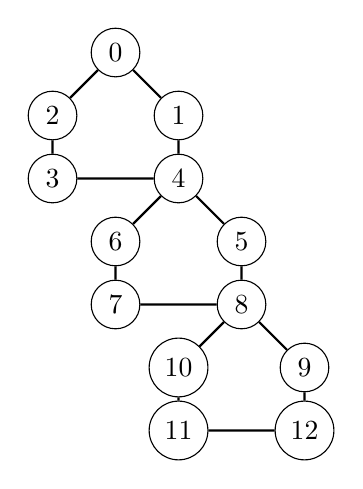
\begin{tikzpicture}
  [scale=.8,auto=left,every node/.style={circle,draw}]
  \node (n0) at (3,18) {0};
  \node (n1) at (4,17)  {1};
  \node (n2) at (2,17)  {2};
  \node (n3) at (2,16) {3};
  \node (n4) at (4,16)  {4};
  \node (n5) at (5,15)  {5};
  \node (n6) at (3,15) {6};
  \node (n7) at (3,14) {7};
  \node (n8) at (5,14) {8};
  \node (n9) at (6,13) {9};
  \node (n10) at (4,13) {10};
  \node (n11) at (4,12) {11};
  \node (n12) at (6,12) {12};

  \foreach \from/\to in {n0/n1, n0/n2, n2/n3, n3/n4, n1/n4, n4/n6, n4/n5, n5/n8, n6/n7, n7/n8, n8/n10, n8/n9, n10/n11, n11/n12, n9/n12}
    \draw [thick] (\from) -- (\to);

\end{tikzpicture}
\end{center}

\caption{Diagonal gluing with $n=5$, $k=3$.}
\label{fig:graph2}

\end{figure}


Instead of using the same transition probabilities as before, we use a \textbf{modified lazy random walk} \label{ref:modlrw} on the Markov chain. 
\begin{definition}
The \textbf{modified lazy random walk} is the lazy random walk with transition probabilities modified so that the stationary distribution is uniform.
\end{definition}
For the diagonally glued graph, the modified lazy random walk will have transition probabilities
\[ P(x,y) = \begin{cases} \frac{1}{8} \ \ \text{ if } y \in N(x), \\
\frac{1}{8} \big(4 - |N(x)| \big) + \frac{1}{2} \ \ \text{ if } y = x,\\
0 \ \ \text{ otherwise.} 
\end{cases}\]


\begin{proposition}
We now consider $n =5$. We have a coupling so that if $\tau$ is the amount of time it takes two walkers to coalesce, then 
\[ \max_{x, y \in \Omega} \mathbf{E}(\tau \ | \ X_0 = x, Y_0 = y) \leq 24k^2 - \frac{528}{25}k + \frac{25}{4}.  \]
Furthermore,
\[ t_{\text{mix}}(\epsilon) \leq \frac{24 k^2}{\epsilon} - \frac{528}{25 \epsilon} k + \frac{25}{4 \epsilon}.\]
\end{proposition}

\begin{proof}

We first define the coupling procedure. Take two random walkers, denoted by $\{X_t\}$ and $\{Y_t\}$, and let them move randomly until they are coupled at the same relative position on the pentagon. To be precise on same relative position, we will need to outline a labeling procedure. For $k \geq 2$, label each corner vertex by multiples of $4$ increasing. Arbitrarily choose some vertex distance $2$ away from the first corner vertex (the corner vertex we labeled as $4$) to be $0$. Label the vertex adjacent to both $0$ and $4$ as $1$. Along the other path to $4$, label the vertex closest to $0$ as $1$ and the vertex closest to $4$ which has not been labeled as $3$. Follow the same procedure for the remaining pentagons; that is, for vertices between $4t$ and $4(t+1)$, label the vertex distance one from both $4t$ and $4(t+1)$ as $4t+1$, label the vertex closest to $4t$ thats not labeled as $4t+2$, and the remaining vertex on the pentagon as $4t+3$. Then two random walkers are on the same relative position if the labels of the vertices they are on are in the same class modulo $4$. 

We will define $h$ as in Proposition \ref{prop:2}. That is, 
\[h(v) = \rho(v,0).\]
We assume again that $h(X_t) \leq h(Y_t)$ without loss of generality. Notice, however, we cannot do the same quotient Markov chain argument as before. This is because vertices which are within the same height class will not necessarily have the same transition probabilities to other vertices in other height classes. As a result, we have to preform a different sort of procedure. Instead, we will have that the walkers will then move in the same directions until we have $h(X_t) = 0$ or until $h(Y_t) = 4k$. 

From there, we shift our coupling to a different kind of coupling. This coupling will have a few different cases: if the walkers are in the same position, they coalesce and from then on they move the same direction; if the walkers are in the same position relative to the pentagon (i.e., they are in the same class determined by their distances away from both glued points), then they move together relative to their respective pentagons; if they are in different classes, we have that they move according to the table in Figure \ref{tb:move1} (for simplicity, if there are not enough rows for the corresponding paths then this means just repeat staying at the respective vertex). For vertices beyond $7$, using the labeling procedure outlined in the first paragraph, take your vertices labels modulo $4$ and proceed according to the table (if your vertex is congruent to $0$ modulo $4$ and is a glued vertex, then treat it like $4$).

The reason for defining the coupling procedure this way is to preserve the property that $h(X_s) \leq h(Y_s)$. This allows us to focus on one walker, which is simpler than trying to focus on both. This leads us to the following proposition.

\begin{figure}

\begin{center}
 \begin{tabular}{||c c c c c c c c c c||} 
 \hline
 (0,1) & (0,2) & (0,3) & (0,4) & (1,2) & (1,3) & (1,4) & (2,3) & (2,4) & (3,4)\\ [0.5ex] 
 \hline\hline
 (1,1) & (0,0) & (1,4) & (0,1) & (0,0) & (0,2) & (0,1) & (3,3) & (0,1) & (2,1)\\ 
 \hline
 (0,0) & (2,2) & (2,2) & (0,3) & (4,3) & (1,3) & (4,4) & (2,2) & (3,3) & (4,4)\\
 \hline
 (2,4) & (1,3) & (0,3) & (0,4) & (1,2) & (4,4) & (1,3) & (0,4) & (2,4) & (3,3)\\
 \hline
 (0,1) & (0,2) & - & (1,5) & - & - & (1,5) & (2,3) & (2,5) & (3,5)\\
 \hline
 - & - & - & (2,6) & - & -  & (1,6) & - & (2,6) & (3,6)\\ [1ex]

 \hline
\end{tabular}
\end{center}

\begin{center}
 \begin{tabular}{||c c c ||} 
 \hline
 (4,5) & (4,6) & (4,7) \\ [0.5ex] 
 \hline\hline
 (1,4) & (5,7) & (5,8) \\ 
 \hline
 (6,8) & (6,6) & (6,6) \\
 \hline
 (5,5) & (1,6) & (3,7) \\
 \hline
 (4,5) & (3,4) & (1,7) \\
 \hline
 - & - & (4,7) \\ [1ex]

 \hline
\end{tabular}
\end{center}
\caption{Locations and destinations of $(X_t, Y_t)$ on the pentagon.}
\label{tb:move1}
\end{figure}


\begin{claim}
For the coupling described above, once $X_s = 0$ and $Y_t = 4j$ for $0 < j < k-1$, we get $h(X_s) \leq h(Y_s)$ for all $s \geq t$. In particular, we get $X_s = Y_s$ once $h(Y_s) = 0$.
\end{claim}

\begin{proof}
We show a similar statement; that is, if $h(X_k) \leq h(Y_k)$ for all $k \leq t$, then $h(X_{t+1}) \leq h(Y_{t+1})$ for all possible choices of $X_{t+1}, Y_{t+1}$. We proceed by induction. The base case of $X_t = 0$ and $Y_t = 4j$ for $0 < j < K$ is true. Assume that $s$ is the first instance where this does not hold; that is, $h(X_t) \leq h(Y_t)$ for all $t \leq s$, but $h(X_{s+1})$ may be larger than $h(Y_{s+1})$. While one would normally need to consider many different cases, using Figure \ref{tb:move1} and the coupling procedure outline above, we see that the only position where $h(X_t) \leq h(Y_t)$ but $h(X_{s+1})$ may be larger on the first pentagon is at $(4,3)$ (read $X_s = 4$, $Y_s = 3$). The strategy will be to work backwards and show that it is actually impossible to reach this position from the starting configuration.

Working backwards, we see that $X_{s-1} = 1$ or $3$ and $Y_{s-1} = 2$ or $4$. If $X_{s-1} = 1$, then we have $(1,2)$ or $(1,4)$ as options. If the walkers are at $(1,2)$, we see that they either coalesce or they go to $(4,3)$, and so this is a possibility. We see that at $(1,4)$ they cannot reach $(4,3)$, and so this is fine. We see that $(3,2)$ results in a contradiction, and so we ignore this case. This leaves $(3,4)$ as an option, but as we can see from the table this does not result in $(4,3)$ and so we exclude it.

In order for $X_{s-1} = 1$, we need $X_{s-2} = 0$ or $X_{s-2} = 4$, and likewise for $Y_{s-1} = 2$ we need $Y_{s-2} = 0$ or $Y_{s-2} = 3$. At $(0,0)$, the walkers are coalesced and so it's impossible to reach $(1,3)$. At $(0,3)$, we see that according to the table it is impossible for us to move to $(1,2)$, and so we omit it. The case $(4,2)$ again results in a contradiction. $(4,3)$ also results in a contradiction, since this implies that they were at this place before $s$. Thus, we see that at the start pentagon it is impossible to reach the case $(4,3)$.

We now consider a pentagon between two glued points. We see that we run into the same issue. Using Figure \ref{fig:graph2}, we have that $X_{s-1} = 8$ and $Y_{s-1} = 7$ leads to a possibility of $h(X_s) > h(Y_s)$. However, for this to happen, we would need $X_{s-2} = 7$ or $X_{s-2} = 5$. If $X_{s-2} = 7$, this means that $Y_{s-2} = 6$ or $Y_{s-2} = 8$ in order to have it at $7$ at time $s-1$. The case of $Y_{s-2} = 6$ immediately gives us a contradiction, since this implies $h(Y_{s-2}) < h(X_{s-2})$. If $Y_{s-2} = 8$ and $X_{s-2} = 7$, then we see that the walkers are at $(7,8)$, which we treat as $(3,4)$. In such a case, it is impossible to get $(8,7)$ on the next step.

In the other direction, if $X_{s-2} = 5$, then we have either $Y_{s-2} = 6$ or $Y_{s-2} = 8$. Thus, we are at either $(5,6)$ or $(5,8)$. If we're at $(5,6)$, we treat it as $(1,2)$, and so we see that it is possible to reach $(8,7)$ according to the table. If the walkers are at $(5,8)$, we see that it is impossible; treating this as $(1,4)$, we have that they must coalesce or we're at $(5,7)$ at $s-1$, which prevents this case.

We then see that in order to get $X_{s-2} = 5$ and $Y_{s-2} = 6$, we must have either $X_{s-3} = 4$ or $X_{s-3} = 8$ and $Y_{s-3} = 7$ or $Y_{s-3} = 4$. We notice that by the table, it is impossible to reach $(5,6)$ from $(4,7)$, and so we are fine. If $X_{s-3} = Y_{s-3} = 4$, then it is also impossible, and so we're fine in such a case. If $X_{s-3} = 8$ and $Y_{s-3} = 4$, we run into a contradiction and so we stop. Thus, we have to consider the case $(8,7)$. But this is itself a contradiction, since we assume that it was impossible to have reached this state prior.

Since we have that it holds for the first pentagon, and for all the glued pentagons, the only other case to consider is at the opposite end. However, for the opposite end, we notice that by flipping the coupling we get that $Y_s$ will always be closer to the opposite end, giving us the same result. Thus, it holds for both end pentagons and all other glued pentagons, and so we see that we get $h(X_s) \leq h(Y_s)$ for all $t \geq s$. As a result, once we get $h(Y_s) = 0 = h(X_s)$, we get that they have coalesced.

\end{proof}

With $\tau$ being the amount of time it takes until they coalesce, we set $\tau = \tau_1 + \tau_2$, where $\tau_1$ is the amount of time it takes for them to couple in their respective pentagons and $\tau_2$ is the amount of time it takes for $h(Y_s) = 0$. Using Gambler's ruin (Proposition \ref{prop:gambleruin}) to bound $\tau_1$ above, we have that this is bounded by a constant,
\[ \max_{x,y \in \Omega} \mathbf{E}(\tau_1 \ | \ X_0 = x, Y_0 =y) \leq \frac{25}{4}.\]
The bound for $\tau_2$ is a little more difficult. Using the same labeling strategy as outlined in Figure \ref{fig:graph2} and the prior proof, we find equations for $\mathbf{E}(\tau_2 \ | \ Y_0 = j)$ where $j \equiv 1 \pmod{4}$ and $j \equiv 3 \pmod{4}$. Let $f_i = \mathbf{E}(\tau_2 \ | \ Y_0 = i\}$.

\begin{claim}\label{claim:snarl}
Let $g_i$ for $0 < i < k+1$ be the equations for $\mathbf{E}(\tau_2 \ | \ Y_0 = j\}$, $j \equiv 1 \pmod{4}$, where $i$ here represents which pentagon we're looking at, with the origin corresponding to $i=1$ and the final corresponding to $i=k$. Then we have 
\[ g_i = \frac{68 + 48(i-2)}{5} + \frac{2i-1}{2i}f_{4i}\]
for $1 < i < k$ and 
\[ g_1 = 4 + \frac{1}{2}f_4.\]
Likewise, let $h_i$ for $0 < i < k+1$ be the formula for $\mathbf{E}(\tau_2 \ | \ Y_0 = j\}$, $j \equiv 3 \pmod{4}$, where $i$ here represents which pentagon we're looking at, with the origin corresponding to $i=1$ and the final corresponding to $i=k$. Then we have 
\[h_i = \frac{72 + (32)(i-2)}{5} + \frac{3i-1}{3i}f_{4i} \]
for $1 < i < k$ and 
\[h_1 = 8 + \frac{2}{3}f_4. \]
\end{claim}

\begin{proof}
We see that this holds for $i=1,2$ respectively by just plugging these equations in. We preform again an inductive argument. Assuming Claim ~\ref{claim:snarl} holds for $i$ again, we show that the inductive hypothesis holds for $i+1$. Notice that by the recursive assignment we get
\[ f_{4i} = \frac{1}{8}(1+g_i) + \frac{1}{8}(1+h_i) + \frac{1}{8}(1+f_{4i+2}) + \frac{1}{8}(1+g_{i+1}) + \frac{1}{2}(1+f_{4i}), \]
\[ g_{i+1} = \frac{1}{8}(1+f_{4i}) + \frac{1}{8}(1+f_{4(i+1)}) + \frac{3}{4}(1+g_{i+1}),\]
\[f_{4i+2} = \frac{1}{8}(1+f_{4i}) + \frac{1}{8}(1+h_{i+1}) + \frac{3}{4}(1+f_{4i+2}), \]
\[h_{i+1} = \frac{1}{8}(1+f_{4i+2}) + \frac{1}{8}(1+f_{4(i+1)}) + \frac{3}{4}(1+h_{i+1}). \]
Solving these equations then gives us the desired result, showing that Claim \ref{claim:snarl} indeed holds.
\end{proof}

Using this, we can solve for when our walker is in the opposite corner, which will give us the maximum expected value. Doing so gives us 
\[ \max_{x, y \in \Omega} \mathbf{E}(\tau_2 \ | \ X_0 =x, Y_0 = y) \leq 24k^2 - \frac{528}{25}k. \]
Summing results together gives us
\[ \max_{x, y \in \Omega} \mathbf{E}(\tau \ | \ X_0 = x, Y_0 = y) = \max_{x, y \in \Omega} \mathbf{E}(\tau_1 + \tau_2 \ | \ X_0 = x, Y_0 = y) \leq 24k^2 - \frac{528}{25}k + \frac{25}{4}.\]

\end{proof}

\begin{remark}
The method we used to find the mixing time of the diagonally glued pentagons is not necessarily unique to the pentagon. However, it is not clear how to sufficiently generalize these results so we can find a mixing time for all $n > 5$ without manually going through and preforming the calculation. Further work could explore this, as well as just exploring the case where we use the standard lazy random walk. One might also want to see if there is a completely general coupling on both $n$ even and $n$ odd, giving us a good way to asymptotically measure the mixing time. 
\end{remark}

\begin{figure}
    \begin{center}
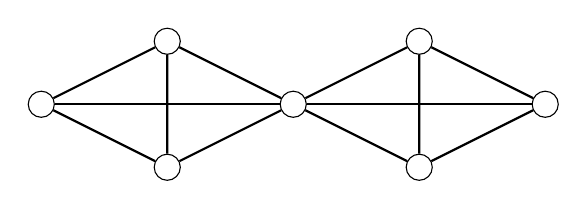
\begin{tikzpicture}
  [scale=.8,auto=left,every node/.style={circle,draw}]
  \node (n0) at (10,10) {};
  \node (n2) at (12,11)  {};
  \node (n3) at (14,10) {};
  \node (n4) at (12,9)  {};
  \node (n5) at (8,11)  {};
  \node (n6) at (6,10) {};
  \node (n7) at (8,9) {};
  
  \foreach \from/\to in {n0/n2, n2/n3, n3/n4, n4/n0, n0/n5, n5/n6, n6/n7, n7/n0, n2/n4, n3/n0, n5/n7, n6/n0}
    \draw [thick] (\from) -- (\to);

\end{tikzpicture}
\end{center}
\caption{Gluing of two complete graphs along a single vertex, with $n=4$.}
\label{fig:graph3}
\end{figure}

\section{Gluings of Complete Graphs} \label{sec:three}

Suppose we took two complete graphs of size $n$ and glued them along a single vertex. An example of this can be seen in Figure \ref{fig:graph3}. The mixing time of this graph is explored using strong stationary times in \cite{LevinPeresWilmer2006} in Example 6.5.1. We do a similar analysis here using coupling.

\begin{proposition}\label{prop:gluedcopies}
The mixing time of the lazy random walk on the graph obtained from gluing two complete graphs along a single vertex is bounded above by 
\[ t_{\text{mix}}(\epsilon) \leq \frac{4n}{\epsilon}.\]
Furthermore, we see that this is actually the same if we glue $k \geq 2$ complete graphs along the same vertex.
\end{proposition}

\begin{proof}
First, couple our walkers in their respective complete graphs as we did with the pentagon example. That is, we want them to be in the same position on their respective graphs. Flip a fair coin and move the walkers $\{X_n\}$ and $\{Y_n\}$ according to the coin flip. Then the probability distribution of the walkers being on the same spot is geometric, with probability $1/(2n)$ of success. Let $\tau_1$ be the amount of time it takes for the walkers to coalesce in this setting. Then since it's geometric, we have 
\[ \max_{x,y \in \Omega} \mathbf{E}(\tau_1 \ | \ X_0 = x, Y_0 = y) \leq 2n.\]
Now, we shift our coupling so that the walkers always move to the same location on their respective graphs. We have that they coalesce when they both hit the center node; that is, the node which all the complete graphs are glued along. The distribution is again geometric, and again we have probability $1/(2n)$ of success. Let $\tau_2$ be the amount of time it takes for the walkers to coalesce here. We get now 
\[ \max_{x, y \in \Omega} \mathbf{E}(\tau_2 \ | \ X_0 =x, Y_0 =y) \leq 2n.\]
Now, let $\tau = \tau_1 + \tau_2$ be the amount of time it takes for the walkers to coalesce entirely. Using the above results, we get 
\[ \max_{x, y \in \Omega} \mathbf{E}(\tau \ | \ X_0 =x, Y_0 =y) = \max_{x,y \in \Omega} \mathbf{E}(\tau_1 + \tau_2 \ | \ X_0 = x, Y_0 = y) \leq 4n, \]
giving us
\[ t_{\text{mix}}(\epsilon) \leq \frac{4n}{\epsilon}.\]
Notice that this same argument works for when we have $k \geq 2$ complete graphs glued along the same vertex (see Figure \ref{fig:graph16}). We have then that the total mixing time is 
\[t_{\text{mix}}(\epsilon) \leq \frac{4n}{\epsilon}. \]
\end{proof}


\begin{figure}

\begin{center}
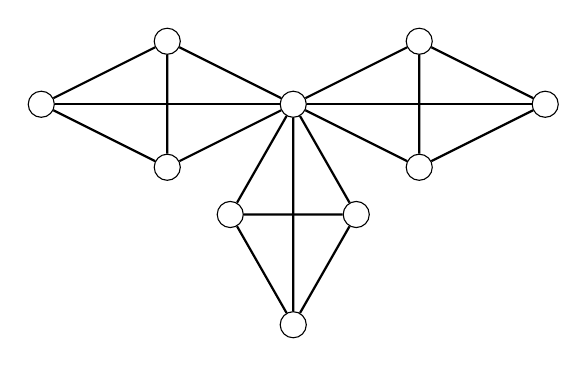
\begin{tikzpicture}
  [scale=.8,auto=left,every node/.style={circle,draw}]
  \node (n0) at (10,10) {};
  \node (n2) at (12,11)  {};
  \node (n3) at (14,10) {};
  \node (n4) at (12,9)  {};
  \node (n5) at (8,11)  {};
  \node (n6) at (6,10) {};
  \node (n7) at (8,9) {};
  \node (n8) at (9,8.25) {};
  \node (n9) at (11,8.25) {};
  \node (n10) at (10, 6.50) {};

  \foreach \from/\to in {n0/n2, n2/n3, n3/n4, n4/n0, n0/n5, n5/n6, n6/n7, n7/n0, n0/n8, n8/n10, n10/n9, n9/n0, n8/n9, n10/n0, n2/n4, n3/n0, n5/n7, n6/n0}
    \draw [thick] (\from) -- (\to);

\end{tikzpicture}
\end{center}
\caption{Gluing complete graphs along a single vertex, with $n=4$, $k=3$.}
\label{fig:graph16}
\end{figure}


We diverge slightly to discuss a coupling on a specific version of a tree. Consider the tree with depth $k$ and three possible paths leading out of its root node $v_*$, and each of the non-vertex non-boundary vertices have degree $2$. An example of this can be seen in Figure \ref{fig:graph5}. We would like to understand the mixing time on this.

\begin{figure}

\begin{center}
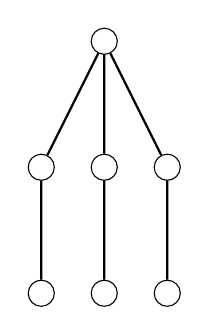
\begin{tikzpicture}
  [scale=.8,auto=left,every node/.style={circle,draw}]
  \node (n0) at (8,10) {};
  \node (n1) at (7,8)  {};
  \node (n2) at (8,8)  {};
  \node (n3) at (9,8) {};
  \node (n4) at (7, 6) {};
  \node (n5) at (8, 6) {};
  \node (n6) at (9, 6) {};
 
  \foreach \from/\to in {n0/n1, n0/n2, n0/n3, n1/n4, n2/n5, n3/n6}
    \draw [thick] (\from) -- (\to);

\end{tikzpicture}
\end{center}
\caption{Tree with three paths of length $k = 2$.}
\label{fig:graph5}
\end{figure}

\begin{proposition}\label{prop:ex}
For the above scenario, we have  
\[ t_{\text{mix}} \leq \frac{3k(k+1)}{\epsilon}.\]
\end{proposition}

\begin{proof}
First, we couple based on height. Here, height will be defined in the standard way; that is, $h(v) = \rho(v, v_*)$. We'll set our transition probabilities to be 
\[ P(x,y) = \begin{cases} \frac{1}{2} \ \text{ if } x = y = v_*, \\ 
\frac{2}{3} \ \text{ if } x = y \neq v_* \text{ and } h(x) \neq k, \\
\frac{5}{6} \ \text{ if } x = y, \ h(x) = k, \\
\frac{1}{6} \ \text{ if } y \in N(x), \\
0 \ \text{ otherwise.}
\end{cases}\]
We'll then only focus on the heights of our walkers. Again, we can push to a quotient Markov chain, using the fact that representatives in each height class have the same probability of moving to a representative in a different heigh class. We can then focus on the chain $\{0, 1, \ldots, k\}$ with transition probabilities nearly the same as above, except the probability of moving down from $0$ is $1/2$. We set the coupling so that the walkers will move in the same direction with respect to height, that is they either move up, down, or stay together, with the caveat that at the root node the walker may sometimes move down while the other walker stays in place. We notice that once the walkers coalesce, they stay coalesced. 

\begin{claim}\label{claim:ajani}
If $h(X_0) \leq h(Y_0)$, then we have $h(X_t) \leq h(Y_t)$ for all $t \geq 0$.
\end{claim}

\begin{proof}
Notice that based on the coupling, if $h(Y_t) = h(Y_{t-1}) \pm 1$ or $h(Y_t) = h(Y_{t-1})$, then $h(X_{t}) = h(X_{t-1}) = \pm 1$ or $h(X_t) = h(X_{t-1})$ as well, with the exception at $h(X_{t-1}) = 0$. Here, we sometimes get $h(X_{t}) = h(X_{t-1}) + 1$ while $h(Y_t) = h(Y_{t-1}) \pm 1$ or $h(Y_t) = h(Y_{t-1})$. We will couple so that if $h(Y_t)$ increases by $1$ then $h(X_t)$ will stay at $0$, if $h(Y_t)$ stays the same then $h(X_t)$ will decrease by $1$, and otherwise $h(X_t)$ will stay at $0$. In such a case, we have coupled the walkers so that they either coalesce or $h(Y_t) > h(X_t)$. Therefore, we get Claim ~\ref{claim:ajani} holds, since once they coalesce they stay coalesced and otherwise we follow the same procedure again.
\end{proof}

As a result of the prior claim, it's sufficient to find out when $h(Y_s) = 0$ to determine when they coalesce. We then repeat the recursive argument. Let $f_i = \mathbf{E}(\tau \ | \ X_0 = i\}$. Then $f_0 = 0$, 
\[f_j = \frac{1}{6}(1+f_{j-1}) + \frac{1}{6}(1+f_{j+1}) + \frac{2}{3}(1+f_j) \]
for $0 < j < k$, and 
\[f_k = \frac{1}{6}(1+f_{k-1}) + \frac{5}{6}(1+f_k). \]

\begin{claim}\label{claim:2}
We have
\[ f_j = 3j + \frac{j}{j+1}f_{j+1}. \]
\end{claim}

\begin{proof}
Again, we see that the base case holds. Assume it holds for $0 < j < k-1$. Then we have  
\[ f_{j+1} = \frac{1}{6}(1+f_j) + \frac{1}{6}(1+f_{j+2}) + \frac{2}{3}(1+f_{j+1}).\]
Substituting in appropriate values and solving this gives us
\[ f_{j+1} = 2(j+1) + \frac{j+1}{j+2}f_{j+2} \]
as desired.
\end{proof}

\begin{claim}
We have $f_i < f_{i+1}$ for all $0 \leq i < k$.
\end{claim}

\begin{proof}
It is a result of Claim \ref{claim:2} and the construction.
\end{proof}

We see that after substituting in the appropriate values from the above claim, we have $f_k = 3k(k+1).$ Combining our claims grants us 
\[ \max_{x, y \in \Omega}\mathbf{E}(\tau \ | \ X_0 =x, Y_0 =y) \leq 3k(k+1), \]
resulting in
\[ t_{\text{mix}}(\epsilon) \leq \frac{3k(k+1)}{\epsilon}.\]
\end{proof}

We now explore the binary tree with depth $k$. The binary tree is generated by attaching two vertices to every vertex of degree one; an example can be seen in Figure \ref{fig:graph6}. We then explore the mixing time of this.

\begin{figure}

\begin{center}
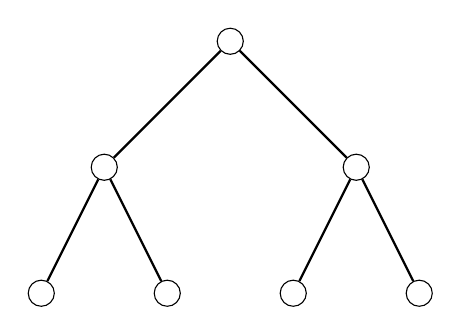
\begin{tikzpicture}
  [scale=.8,auto=left,every node/.style={circle,draw}]
  \node (n0) at (8,10) {};
  \node (n1) at (6,8)  {};
  \node (n2) at (10,8) {};
  \node (n3) at (5, 6) {};
  \node (n4) at (7, 6) {};
  \node (n5) at (9, 6) {};
 \node (n6) at (11, 6) {};
 
  \foreach \from/\to in {n0/n1, n0/n2, n1/n3, n1/n4, n2/n5, n2/n6}
    \draw [thick] (\from) -- (\to);

\end{tikzpicture}
\end{center}
\caption{Binary tree of depth $k = 2$.}
\label{fig:graph6}
\end{figure}

\begin{proposition}\label{prop:binarylazyrw}
For the lazy random walk on the binary tree of depth $n$, we have 
\[ \max_{x,y \in \Omega} \mathbf{E}(\tau \ | \ X_0 = x, Y_0 = y) \leq 6 \cdot 2^n. \]
\end{proposition}

\begin{proof}
The result can be found in Example 5.3.4 in \cite{LevinPeresWilmer2006}. We give the outline of the proof here. Let $h$ again be the distance of a node from the root node; that is, $h(v) = \rho(v, v_*)$. Again, we can push to the quotient Markov chain using the height equivalence class, since transition probabilities between representatives are coherent. Thus, we can instead just consider the Markov chain on this sequence of numbers instead of the actual chain, with transition probabilities derived from the lazy random walk. Then we couple based on the distance from the root; that is, if one walker goes down, then the other walker goes down, and likewise for moving up. Doing so gives us the upper bound of 
\[ \max_{x,y \in \Omega} \mathbf{E}(\tau \ | \ X_0 = x, Y_0 =y) \leq 6 \cdot 2^n.\]
This matches our intuition, since this should be much larger than the result we found in Proposition ~\ref{prop:ex}.
\end{proof}

However, the coupling and argument didn't actually use the fact that there were only two paths leading out of the root node. Suppose we glued another copy of the binary tree of length $k-1$ to the root node of the binary tree of length $k$. Then similar to Proposition ~\ref{prop:gluedcopies}, we see that the mixing time is still the same. 

We now introduce an iterated process for gluing copies of $K_3$ for Proposition ~\ref{prop:elvishmystic}. Throughout, we define an \textbf{open vertex} to be vertices whose degree is $2$. At $k=1$, we simply have the complete graph itself. At $k=2$, we glue a copy of the graph on each vertex. At $k=3$, we glue more copies along each open vertex. One can also think of gluing these copies along the boundary of our new graph. An example of this gluing procedure can be found in Figure ~\ref{fig:graph4}.


One can then ask how we should expect the bound of the mixing time of the modified lazy random walk to behave as we increase $k$. We use the transition matrix introduced in Section \ref{sec:two}; that is, we have 
\[ P(x,y) = \begin{cases} \frac{1}{8} \ \ \text{ if } y \in N(x), \\
\frac{1}{8} \big(4 - |N(x)| \big) + \frac{1}{2} \ \ \text{ if } y = x,\\
0 \ \ \text{ otherwise.} 
\end{cases}\]

Recall again that we do this so that the stationary distribution is uniform.

\begin{proposition} \label{prop:elvishmystic}
For the above scenario, we have that for $k > 1$
\[t_{\text{mix}}(\epsilon) \leq \frac{104}{3 \epsilon} 2^k - \frac{16}{\epsilon}k - \frac{100}{3 \epsilon} \]
\end{proposition}


\begin{figure}

\begin{center}
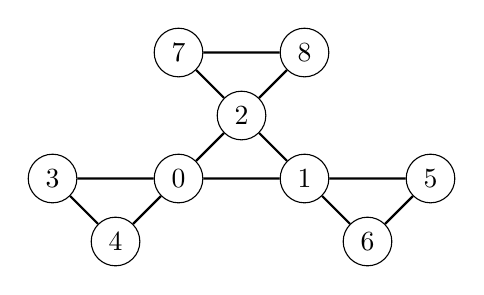
\begin{tikzpicture}
  [scale=.8,auto=left,every node/.style={circle,draw}]
  \node (n0) at (8,10) {0};
  \node (n1) at (10,10)  {1};
  \node (n2) at (9,11)  {2};
  \node (n3) at (12,10) {5};
  \node (n4) at (11, 9) {6};
  \node (n5) at (6, 10) {3};
  \node (n6) at (7, 9) {4};
  \node (n7) at (8, 12) {7};
  \node (n8) at (10,12) {8};

  \foreach \from/\to in {n0/n5, n5/n6, n6/n0, n0/n1, n1/n4, n4/n3, n3/n1, n1/n2, n2/n7, n7/n8, n8/n2, n2/n0}
    \draw [thick] (\from) -- (\to);

\end{tikzpicture}
\end{center}

\caption{Expansion gluing $n=3$, $k=2$.}
\label{fig:graph4}
\end{figure}

\begin{proof}
Let our random walkers start anywhere on the graph. We couple first based on the distance away from the first triangle. We change our height function to be 
\[h(v) = \min_{x \in \{0,1,2\}} \{\rho(x,v)\} \]
where $0,1,2$ will be the vertices on the origin, or center, triangle, as seen in Figure \ref{fig:graph4}. We have then transformed our random walk on the large graph to a random walk on $\{0, 1, \ldots, k\}$ such that when $h(X_t) = h(Y_t)$, we have $h(X_s) = h(Y_s)$ for all $s \geq t$. Imagine this set up on a line, with the leftmost position being the origin triangle and the rightmost triangle being the boundary. Then the probability of going left, or going towards the origin triangle, is $1/8$, the probability of going right, or away from the origin triangle, is $1/4$, and the probability of staying in place is $5/8$. We also have that trying to move left or right at the endpoints results in staying in place respectively. We will also couple our walks so that whenever $X_t$ goes left, right, or stays in place, then $Y_t$ also goes left, right, or stays in place respectively. It is sufficient then to find the expected amount of time it takes the walker with the highest height to hit $0$. Without loss of generality, take this walker to be $\{Y_t\}$.

Let $\tau$ be the amount of time it takes for a walker to hit $0$. We set $f_j = \mathbf{E}(\tau \ | \ X_0 = j)$. We have $f_0 = 0$, 
\[f_k = \frac{7}{8}(1+f_k) + \frac{1}{8}(1+f_{k-1}), \]
and
\[f_j = \frac{5}{8}(1 + f_j) + \frac{1}{4}(1+f_{j+1}) + \frac{1}{8}(1+f_{j-1}) \]
for $0 < j < k$. 

\begin{claim}\label{claim:free}
We have
\[f_j =  \frac{8(2^{j+1}-j-2)}{2^{j+1}-1} + \frac{2^{j+1}-2}{2^{j+1}-1}f_{j+1}. \]
\end{claim}

\begin{proof}
Solving for $f_1$ grants us 
\[f_1 = \frac{8}{3} + \frac{2}{3}f_2, \]
as desired. Assume Claim \ref{claim:free} holds for $j$, $0 < j < k-1$. Then we must show the inductive hypothesis holds for $j +1$. We have
\[f_j =  \frac{8(2^{j+1}-j-2)}{2^{j+1}-1} + \frac{2^{j+1}-2}{2^{j+1}-1}f_{j+1} \]
and
\[f_{j+1} = \frac{5}{8}(1+f_{j_1}) + \frac{1}{4}(1+f_{j+2}) + \frac{1}{8}(1+f_j). \]
Substituting in appropriate values gives
\[f_{j+1} =  \frac{8(2^{j+2}-(j+1)-2)}{2^{j+2}-1} + \frac{2^{j+2}-2}{2^{j+2}-1}f_{j+2}. \]
\end{proof}

\begin{claim}
We have $f_i < f_{i+1}$ for all $0 \leq i < k$.
\end{claim}

\begin{proof}
This is a result of Claim ~\ref{claim:free} and the construction itself.
\end{proof}

The prior claims give us
\[f_k = 2^{k+4} - 16 - 8k. \]
So the expected amount of time for the walkers to coalesce is bounded above by $f_k$.

\begin{figure}

\begin{center}
 \begin{tabular}{| c ||} 
 \hline
 (0,1)\\  
 \hline\hline
 (0,0) \\
 \hline
 (1,1) \\ 
 \hline
 (2,2)\\
 \hline
 (3,5) \\
  
 \hline
 (4,6)\\ 

 \hline
\end{tabular}
\end{center}
\caption{Locations and destinations of $(X_t = 0, Y_t = 1)$, with top row being the initial states and remaining being the coupled moves.}
\label{tb:move2}
\end{figure}

Now, we create another coupling. The walkers move the same direction on their respective triangles until they reach the origin triangle; that is, once $\rho(X_t, Y_t) \leq 1$. We then have that if they try to move to one of the other two vertices on the origin triangle or stay in place, then they coalesce. If they otherwise move backwards, then they move backwards identically. An example of this can be found in Figure \ref{tb:move2}, with reference to Figure \ref{fig:graph4}. This then gives us a random walk on the graph of their distance $\rho(X_t, Y_t) = \{0,1,3,5,\ldots, 2k+1\}$, with absorption at $0$, a $3/4$ chance of going to $0$ from $1$, a $1/4$ chance of going from $1$ to $3$, and the rest of the chain remains identical to the quotient chain mentioned prior. To make things easier, we'll rewrite this instead as $\{0,1,2,3,\ldots,k,k+1\}$ (the $k$ here is important, and as a result we cannot use a different variable here in its stead). We then want to find the expected amount of time until they coalesce at $0$. Again, we set up a series of equations with $f_j = \mathbf{E}(\tau \ | \ X_0 = j)$, and we see $f_0 = 0$, 
\[f_1 = \frac{3}{4} + \frac{1}{4}(1 + f_2), \]
\[f_{k+1} = \frac{7}{8}(1+f_{k+1}) + \frac{1}{8}(1+f_{k}), \]
and
\[f_j = \frac{5}{8}(1 + f_j) + \frac{1}{4}(1+f_{j+1}) + \frac{1}{8}(1+f_{j-1}), \]
for $1 < j < m+1$. 
\begin{claim}\label{claim:jund}
We have
\[ f_j = \frac{56 \cdot 2^{j-1}-24j-28}{7 \cdot 2^{j-1}-3} + \bigg(\frac{7(2^{j-1})-6}{7(2^{j-1})-3}\bigg) f_{j+1}\]
for $0 < j < k$.
\end{claim}

\begin{proof}
We proceed by induction again. We see that substituting in $j=1$ gives us 
\[f_1 = 1 + \frac{1}{4}f_2, \]
as required. We now assume Claim \ref{claim:jund} holds for $j$, and show it holds for $j+1$. We have 
\[f_j =  \frac{56 \cdot 2^{j-1}-24j-28}{7 \cdot 2^{j-1}-3} + \bigg(\frac{7(2^{j-1})-6}{7(2^{j-1})-3}\bigg) f_{j+1}\]
and
\[f_{j+1} = \frac{5}{8}(1+f_{j+1}) + \frac{1}{4}(1+f_{j+2}) + \frac{1}{8}(1+f_j). \]
Substituting in the appropriate values and solving for $f_{j+1}$, we have
\[ f_{j+1} = \frac{56 \cdot 2^{j}-24(j+1)-28}{7 \cdot 2^{j}-3} + \bigg(\frac{7(2^{j})-6}{7(2^{j})-3}\bigg) f_{j+2} \]
as desired.
\end{proof}

\begin{claim}
We again get $f_j < f_{j+1}$ for $0 \leq j < k+1$.
\end{claim}

\begin{proof}
Again, a result from the prior claim and the construction.
\end{proof}

\noindent We find that 
\[f_{k+1} = \frac{112}{3} 2^{k-1} - 8k - \frac{52}{3}. \]
So the expected time for the two random walkers to coalesce once they've coupled using the prior couple is bounded by $f_{k+1}$. Hence, if $\tau$ is the amount of time for them to couple, we've found that 
\[\max_{x,y \in \Omega} \mathbf{E}(\tau \ | \ X_0 = x, Y_0 = y) \leq \frac{104}{3} 2^k - 16k - \frac{100}{3}, \]
where $k$ is the number of times we've iterated the gluing procedure. We get then
\[t_{\text{mix}}(\epsilon) \leq \frac{104}{3 \epsilon} 2^k - \frac{16}{\epsilon}k - \frac{100}{3 \epsilon} \]
as desired.
\end{proof}

\section{Mixing Times on Nice Classes of 3-Regular Graphs} \label{sec:four}

\begin{figure}

\begin{center}
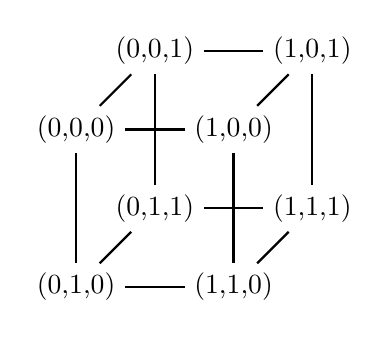
\begin{tikzpicture}
  
  \node (n0) at (4,4) {(1,0,0)};
  \node (n1) at (4,2) {(1,1,0)};
  \node (n2) at (2,2) {(0,1,0)};
  \node (n3) at (2,4) {(0,0,0)};

  \node (n4) at (3,5) {(0,0,1)};
  \node (n5) at (5,5) {(1,0,1)};
  \node (n6) at (3,3) {(0,1,1)};
  \node (n7) at (5,3) {(1,1,1)};

  \path[]
  (n0) [-, thick] edge node [] {} (n3);
  \path[] (n3) [-, thick] edge node [] {} (n2);
  \path[] (n3) [-, thick] edge node [] {} (n4);
\path[] (n2) [-, thick] edge node [] {} (n1);
\path[] (n2) [-, thick] edge node [] {} (n6);
\path[] (n4) [-, thick] edge node [] {} (n6);
\path[] (n4) [-, thick] edge node [] {} (n5);
\path[] (n6) [-, thick] edge node [] {} (n7);
\path[] (n0) [-, thick] edge node [] {} (n1);
\path[] (n0) [-, thick] edge node [] {} (n5);
\path[] (n5) [-, thick] edge node [] {} (n7);
\path[] (n1) [-, thick] edge node [] {} (n7);
\end{tikzpicture}
\end{center}
\caption{3-dimensional hypercube.}
\label{fig:graph7}
\end{figure}

\begin{figure}
\begin{center}
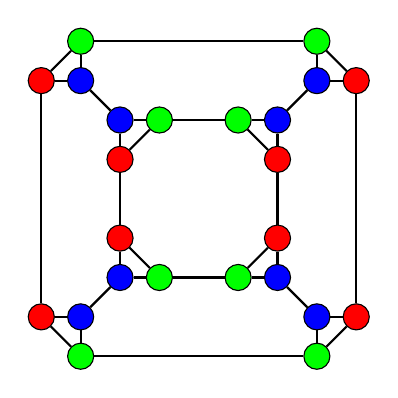
\begin{tikzpicture}[updown node/.style={circle,fill=red, draw, minimum size=0.02cm}, leftright node/.style={circle,fill=green,   draw, minimum size=0.02cm}, inout node/.style={circle, fill=blue, draw, minimum size = 0.02cm}]
% inner
%triangle 1

% i/o
\node[inout node] (n0) at (10, 10) {};

% u/d
\node[updown node] (n1) at (10,10.5) {};

%l/r
\node[leftright node] (n2) at (10.5,10) {};

% triangle 2

%l/r
\node[leftright node] (n3) at (11.5,10) {};

%i/o
\node[inout node] (n4) at (12,10) {};

%u/d
\node[updown node] (n5) at (12, 10.5) {};

% triangle 3

%u/d
\node[updown node] (n6) at (12, 11.5) {};

%i/o
\node[inout node] (n7) at (12, 12) {};

%l/r
\node[leftright node] (n8) at (11.5, 12) {};

% triangle 4

%l/r
\node[leftright node] (n9) at (10.5, 12) {};

%i/o
\node[inout node] (n10) at (10, 12) {};

%u/d
\node[updown node] (n11) at (10, 11.5) {};

% outer
%triangle 5

% i/o
\node[inout node] (n12) at (9.5,9.5) {};

%u/d
\node[updown node] (n13) at (9, 9.5) {};

%l/r
\node[leftright node] (n14) at (9.5,9) {};

%triangle 6

%i/o
\node[inout node] (n15) at (12.5, 9.5) {};

%u/d
\node[updown node] (n16) at (13, 9.5) {};

%l/r
\node[leftright node] (n17) at (12.5, 9) {};

%triangle 7

%i/o
\node[inout node] (n18) at (12.5, 12.5) {};

%u/d
\node[updown node] (n19) at (13, 12.5) {};

%l/r
\node[leftright node] (n20) at (12.5, 13) {};

%triangle 8

% i/o
\node[inout node] (n21) at (9.5, 12.5) {};

%l/r
\node[leftright node] (n22) at (9.5, 13) {};

%u/d
\node[updown node] (n23) at (9, 12.5) {};

\path[] 
% inner cycle
% triangle 1
(n0) [-, thick] edge node [] {} (n1)
(n1) [-,thick] edge node [] {} (n2)
(n2) [-,thick] edge node [] {} (n0)

% triangle 1 -> triangle 2
(n2) [-,thick] edge node [] {} (n3)

% triangle 2
(n3) [-,thick] edge node [] {} (n4)
(n4) [-,thick] edge node [] {} (n5)
(n5) [-,thick] edge node [] {} (n3)

% triangle 2 -> triangle 3
(n5) [-,thick] edge node [] {} (n6)

% triangle 3
(n6) [-,thick] edge node [] {} (n7)
(n7)[-,thick] edge node [] {} (n8)
(n8)[-,thick] edge node [] {} (n6)

% triangle 3 -> triangle 4
(n8)[-,thick] edge node [] {} (n9)

% triangle 4
(n9)[-,thick] edge node [] {} (n10)
(n10)[-,thick] edge node [] {} (n11)
(n11)[-,thick] edge node [] {} (n9)

% triangle 4 -> triangle 1
(n11) [-, thick] edge node [] {} (n1)

% inner cycle -> outer cycle
(n0) [-,thick] edge node [] {} (n12)
(n4) [-,thick] edge node [] {} (n15)
(n7) [-,thick] edge node [] {} (n18)
(n10) [-,thick] edge node [] {} (n21)

% triangle 5
(n12) [-,thick] edge node [] {} (n13)
(n13) [-,thick] edge node [] {} (n14)
(n14) [-,thick] edge node [] {} (n12)

% triangle 6
(n15) [-,thick] edge node [] {} (n16)
(n16) [-,thick] edge node [] {} (n17)
(n17) [-,thick] edge node [] {} (n15)

% triangle 7
(n18) [-,thick] edge node [] {} (n19)
(n19) [-,thick] edge node [] {} (n20)
(n20) [-,thick] edge node [] {} (n18)

% triangle 8
(n21) [-,thick] edge node [] {} (n22)
(n22) [-,thick] edge node [] {} (n23)
(n23) [-,thick] edge node [] {} (n21)

% triangle 5 -> triangle 6
(n14) [-,thick] edge node [] {} (n17)

%triangle 6 -> triangle 7
(n16) [-,thick] edge node [] {} (n19)

% triangle 7 -> triangle 8
(n20) [-,thick] edge node [] {} (n22)

% triangle 8 -> triangle 5
(n23) [-, thick] edge node [] {} (n13)
;

\end{tikzpicture}
\end{center}
    \caption{$3$-dimensional triangulated hypercube.}
    \label{fig:graph17}
\end{figure}



Consider the space of binary strings of length $n$; that is, let 
\[\Omega = \{0,1\}^n = \left\{v = (v_1, \ldots, v_n) \ : \ v_i \in \{0,1\}\right\}.\] 
\begin{definition}
We define the \textbf{Hamming weight} on this space to be a function $H : \Omega \rightarrow \{0, \ldots, n\}$ such that 
\[ H(v) = \sum_{i=1}^n v_i.\]
\end{definition}
In other words, we sum the components of this vector. 
\begin{definition}
We form the \textbf{n-dimensional Hypercube} by taking the space $\Omega$ to be the set of vertices for our graph, and we connect an edge between $v, w \in \Omega$ if 
\[|H(v) - H(w)| = 1.\]
\end{definition}
We have that the $3$-dimensional Hypercube forms a very nice $3$-regular graph, in that it is \textbf{vertex transitive}.

\begin{definition}
A graph $G$ is \textbf{vertex transitive} if, for any two vertices $v_1$, $v_2$, there is some map $f: G \rightarrow G$ preserving edge-vertex connectivity (also referred to as a \textbf{graph automorphism}) with
\[f(v_1) = v_2. \]
\end{definition}

\begin{remark}
All of the graphs mentioned in this section will be vertex transitive. This may be important (see the Question ~\ref{question:one}), however we do not really use this property in finding any of the mixing times themselves. When referring to ``nice class of graphs,'' we mean a family of vertex transitive $3$-regular graphs which are easily describable.
\end{remark}

An example of this graph can be seen in Figure \ref{fig:graph7}. The mixing time of the lazy random walk on this graph is well understood to be 
\[ t_{\text{mix}} \leq n \log(n) - n \log(\epsilon)\]
as seen in Example 5.3.1 in \cite{LevinPeresWilmer2006}. 
% Put it in the appendix as well?
We would like to understand the behavior of the modified lazy random walk on the \textbf{triangulated} $3$-dimensional hypercube. By triangulated, we mean replacing each vertex with a copy of $K_3$ and attaching corresponding edges. An example can be seen of the process can be seen in Figures \ref{fig:graph8} and the triangulated version of the $3$-dimensional hypercube can be seen in \ref{fig:graph17}. 

\begin{proposition}
For the lazy random walk on the triangulated $3$-dimensional hypercube, we have 
\[ t_{\text{mix}}(\epsilon) \leq \frac{42}{\epsilon}.\]
\end{proposition}


\begin{figure}

    \begin{center}
\begin{tikzpicture}[main node/.style={circle,draw}]
  
  \node[main node] (n0) at (2,0) {};
  \node (n1) at (0,0) {};
  \node (n2) at (2,2) {};
  \node (n3) at (4,0) {};

  \path[] (n0) [-, thick] edge node [] {} (n1);
   \path[] (n0) [-, thick] edge node [] {} (n2);
   \path[] (n0) [-, thick] edge node [] {} (n3);
\end{tikzpicture}
$\rightarrow$
\begin{tikzpicture}[main node/.style={circle,draw}]
  
  \node[main node] (n0) at (1,0) {};
  \node[main node] (n4) at (3,0) {};
  \node[main node] (n5) at (2,1) {};
  \node (n1) at (0,0) {};
  \node (n2) at (2,2) {};
  \node (n3) at (4,0) {};

  \path[] (n0) [-, thick] edge node [] {} (n1);
   \path[] (n2) [-, thick] edge node [] {} (n5);
   \path[] (n3) [-, thick] edge node [] {} (n4);
   \path[] (n0) [-, thick] edge node [] {} (n4);
 \path[] (n0) [-, thick] edge node [] {} (n5);
 \path[] (n4) [-, thick] edge node [] {} (n5);
\end{tikzpicture}
\end{center}
    \caption{Triangulating a vertex on a $3$-regular graph}
    \label{fig:graph8}
\end{figure}

\begin{proof}
Recall that the lazy random walk on this graph will be 
\[P(x,y) = \begin{cases} \frac{1}{2} \ \text{ if } x = y, \\ \frac{1}{6} \ \text{ if } y \in N(x), \\ 0 \text { otherwise.} \end{cases} \]
Notice that the vertices on our triangle correspond to dimensions, as can be seen in Figure \ref{fig:graph17}. That is, we have that the blue vertices correspond to moving in and out, the red vertices correspond to moving up and down, and the green vertices correspond to moving left and right in Figure \ref{fig:graph17}. Assume that our walkers do not match in any dimensions at their start. Then the expected amount of time until they match in some dimension is a geometric random variable with a probability of success being $1/6$. The expected time for this is then $6$. Now, our walkers will move together in the dimension that they have matched up in, and will move independently on either two dimensions. We now want to measure the expected amount of time until our walkers match in another dimension. We now have three states to consider; if our walkers are on the vertex color they have matched in, if they are on a new color they have not yet matched in, and if they have coalesced in a new color or dimension. We denote these by $2$, $1$, and $0$ respectively. Doing so now transforms our Markov chain to a walk on $\{0,1,2\}$. Let $\tau'$ be the amount of time it takes until our walker on this new chain reaches $0$. Then we set $f_i = \mathbf{E}(\tau' \ | \ X_0 = i)$, giving us $f_0 = 0$, 
\[f_1 = \frac{1}{6} + \frac{2}{3}(1+f_1) + \frac{1}{6}(1+f_2), \]
and
\[f_2 = \frac{2}{3}(1+f_2) + \frac{1}{3}(1+f_1). \]
Solving this sequence of equations gives $f_2 = 12$ as our upper bound for this portion. Now with our walkers matching in $2$ dimensions, we want to see how long it takes until they match in the third, and therefore coalesce. We again have the three options we had before; our walkers are on a vertex in which they already match in dimension, they are on a vertex which they do not match in dimension, or they have coalesced in this final dimension. Again, we represent these states as $2$, $1$, and $0$. We have that our Markov chain is a walk on $\{0,1,2\}$, with $0$ as the absorbing state. Using the same notation as before, we have $f_0 = 0$,
\[f_1 = \frac{1}{6} + \frac{1}{3}(1+f_2) + \frac{1}{2}(1+f_1), \]
and
\[ f_2 = \frac{5}{6}(1+f_2) + \frac{1}{6}(1+f_1).\]
Solving this series of equations gives us $f_2 = 24$, and so we have an upper bound of $24$. If $\tau$ is the amount of time until the walkers coalesce, then we have a bound of 
\[\max_{x,y \in \Omega} \mathbf{E}(\tau \ | \ X_0 = x, Y_0 =y) \leq 6 + 12 + 24 =  42\]
as desired.
\end{proof}

This then begs the question of whether or not there is some relation between the mixing time of the modified random walk on the triangulated graph and the mixing time of the modified walk on the $3$-regular graphs. To explore this, we first study the \textbf{prism graph}. 

\begin{definition}
The \textbf{prism graph} on $2n$ vertices is constructed by taking two cycles of length $n$ and attaching edges between corresponding vertices. Notationally, we have $G = (V,E)$ is the prism graph if
\[ V = \{(a,b) \ | \ a \in \{0,1\}, b \in \{0, \ldots, n-1\} \}, \]
\[ E = \left\{\left((a,b), (c,d)\right) \ | \ a = c, b = d \pm 1 \Mod{n} \right\}.\]
An example of a prism graph can be seen in Figures \ref{fig:graph7} and \ref{fig:graph9}.  
\end{definition}

\begin{figure}
   
    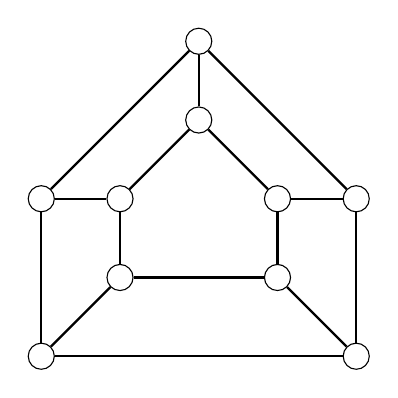
\begin{tikzpicture}[main node/.style={circle,draw}]
  
  \node[main node] (n0) at (2,2) {};
  \node[main node] (n1) at (2,3) {};
  \node[main node] (n2) at (3,4) {};
  \node[main node] (n3) at (4,3) {};
  \node[main node] (n4) at (4,2) {};
  \node[main node] (n5) at (1,1) {};
  \node[main node] (n6) at (1,3) {};
  \node[main node] (n7) at (3,5) {};
 \node[main node] (n8) at (5,3) {};
 \node[main node] (n9) at (5,1) {};
 \path[]
 (n0) [-, thick] edge node [] {} (n1)
 (n1) [-] edge node [] {} (n2)
 (n2) [-] edge node [] {} (n3)
 (n3) [-] edge node [] {} (n4)
 (n0) [-] edge node [] {} (n4)
 (n0) [-] edge node [] {} (n5)
 (n5) [-] edge node [] {} (n6)
 (n6) [-] edge node [] {} (n7)
 (n7) [-] edge node [] {} (n8)
 (n8) [-] edge node [] {} (n9)
 (n9) [-] edge node [] {} (n5)
 (n1) [-] edge node [] {} (n6)
 (n2) [-] edge node [] {} (n7)
 (n3) [-] edge node [] {} (n8)
 (n4) [-] edge node [] {} (n9);
\end{tikzpicture}
 \caption{Prism graph of size $10$}
    \label{fig:graph9}
\end{figure}

\begin{proposition}\label{prop:funsies}
For the lazy random walk on the prism graph of size $n$, we have 
\[t_{\text{mix}} \leq \frac{3 n^2}{16 \epsilon} + \frac{6}{\epsilon} \]
\end{proposition}

\begin{proof}
We first couple based on whether our walkers are both on the inner or outer cycles. Flipping a coin to decide which walker moves and letting them move wherever possible, we see that this it is a geometric random variable until our walkers match in cycle. Since there is a probability of $1/6$ of the walker moving into the same cycle at each step, we have that the expected amount of time is $6$. It is now simply a random walk on the cycle with a higher chance of staying in place ($2/3$ chance of staying in place, and $1/6$ chance of going left or right). Running through the process, we have 
\[ f_k = 3k + \frac{k}{k+1} f_   {k+1}\]
leading us to have
\[ f_k = 3k\left(\frac{n}{2}-k\right).\]
Maximizing this gives 
\[ \max_{x,y \in \Omega} \mathbf{E}(\tau \ | \ X_0 = y, Y_0 =y) \leq \frac{3}{16} n^2 + 6\]
as desired.
\end{proof}

This argument lets us also find the mixing time of the \textbf{M\"{o}bius ladder graph}. 

\begin{definition}
The \textbf{M\"{o}bius ladder graph} is formed by doing the same construction as the prism graph, except there's a twist at the bottom. Notationally, we have $G = (V,E)$ is the M\"{o}bius ladder graph of size $2n$ if
\[V = \{ (a,b) \ | \ a \in \{0,1\}, b \in \{0, \ldots, n-1\} \}, \] 
\[E = \{\left((a,b), (c,d)\right) \ | \ a = b \text{ and } b = d \pm 1 \Mod{n}, b \in \{1, \ldots, n-2\} \]
\[ \text{ or } a = 1-b \text{ and } b = d +1 \Mod{n} \text{ if } d = n-1, b = d-1 \Mod{n} \text{ if } d = 0 \}. \]
An example can be seen in Figure \ref{fig:graph11}. Since the M\"{o}bius ladder graph can be unwound, as seen in Figure \ref{fig:graph10}, we could alternatively identify this as 
\[V = \{0, \ldots, 2n-1\} \]
\[E = \left\{(a,b) \ | \ a = b \pm 1 \Mod{2n} \text { or } a = b \pm n \Mod{2n}\right\}. \]
\end{definition}

\begin{figure}
    
    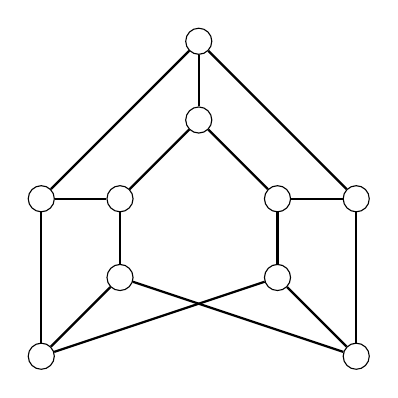
\begin{tikzpicture}[main node/.style={circle,draw}]
  
  \node[main node] (n0) at (2,2) {};
  \node[main node] (n1) at (2,3) {};
  \node[main node] (n2) at (3,4) {};
  \node[main node] (n3) at (4,3) {};
  \node[main node] (n4) at (4,2) {};
  \node[main node] (n5) at (1,1) {};
  \node[main node] (n6) at (1,3) {};
  \node[main node] (n7) at (3,5) {};
 \node[main node] (n8) at (5,3) {};
 \node[main node] (n9) at (5,1) {};
 \path[]
 (n0) [-, thick] edge node [] {} (n1)
 (n1) [-] edge node [] {} (n2)
 (n2) [-] edge node [] {} (n3)
 (n3) [-] edge node [] {} (n4)
 (n0) [-] edge node [] {} (n5)
 (n4) [-] edge node [] {} (n5)
 (n5) [-] edge node [] {} (n6)
 (n6) [-] edge node [] {} (n7)
 (n7) [-] edge node [] {} (n8)
 (n8) [-] edge node [] {} (n9)
 (n9) [-] edge node [] {} (n0)
 (n1) [-] edge node [] {} (n6)
 (n2) [-] edge node [] {} (n7)
 (n3) [-] edge node [] {} (n8)
 (n4) [-] edge node [] {} (n9);
\end{tikzpicture}
\caption{M\"{o}bius ladder graph of size $10$}
    \label{fig:graph11}
\end{figure}


\begin{corollary}\label{cor:one}
For the modified lazy random walk on the M\"{o}bius ladder graph, we have that the mixing time is 
\[ t_{\text{mix}} \leq \frac{3n^2}{16 \epsilon} + \frac{6}{\epsilon}. \]
\end{corollary}

\begin{proof}
Notice that the M\"{o}bius ladder graph can be unwound to get the circulant graph, as seen in Figure \ref{fig:graph10}. We identify two vertices across from one another to be in the same class, that is, vertices $v_1, v_2 \in V$ are in the same class if $v_1 = v_2 + n/2 \Mod{n}$. This pushes our Markov chain to its quotient Markov chain. We see we have a cycle on $n/2$, with modified probability of staying in place as in Proposition \ref{prop:funsies}. Moreover, once coupled in class, we just need to couple in position itself. Flip a coin and move the walker; if it jumps across, we have the walkers coalesce and we win. Otherwise, move the other walkers so that they are still in the same class. Then the probability of the walkers coalescing is a geometric random variable with probability $1/6$, and so we get the same constant factor of $6$ as an upper bound for this latter bound. Summing our two results together gives the result.
\end{proof}

\begin{figure}
    
    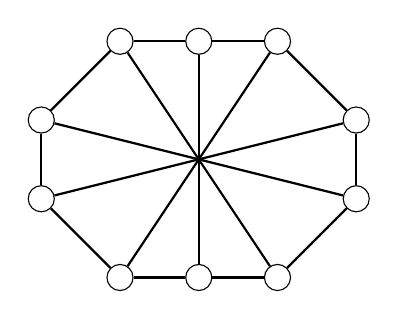
\begin{tikzpicture}[main node/.style={circle,draw}]
  
  \node[main node] (n0) at (3,2) {};
  \node[main node] (n1) at (4,2) {};
  \node[main node] (n2) at (5,2) {};
  \node[main node] (n3) at (6,3) {};
  \node[main node] (n4) at (6,4) {};
  \node[main node] (n5) at (5,5) {};
  \node[main node] (n6) at (4,5) {};
  \node[main node] (n7) at (3,5) {};
  \node[main node] (n8) at (2,4) {};
  \node[main node] (n9) at (2,3) {};
 \path[]
 (n0) [-, thick] edge node [] {} (n5)
 (n1) [-] edge node [] {} (n6)
 (n2) [-] edge node [] {} (n7)
 (n3) [-] edge node [] {} (n8)
 (n4) [-] edge node [] {} (n9)
 (n0) [-] edge node [] {} (n1)
 (n1) [-] edge node [] {} (n2)
 (n2) [-] edge node [] {} (n3)
 (n3) [-] edge node [] {} (n4)
 (n4) [-] edge node [] {} (n5)
 (n5) [-] edge node [] {} (n6)
 (n6) [-] edge node [] {} (n7)
 (n7) [-] edge node [] {} (n8)
 (n8) [-] edge node [] {} (n9)
 (n9) [-] edge node [] {} (n0);
 
\end{tikzpicture}
\caption{Unwound M\"{o}bius ladder graph of size $10$.}
    \label{fig:graph10}
\end{figure}

\begin{proposition}\label{prop:stup}
For the lazy random walk on the triangulated prism graph of size $n$, we have 
\[ t_{\text{mix}}(\epsilon) \leq \frac{15 n^2}{16 \epsilon} + \frac{87}{5\epsilon}.\]
\end{proposition}

\begin{proof}
We again want to start by coupling based on which cycle (either inner or outer) we are in. Letting the walkers move independently of one another, we wait until they occupy the same location relative to their triangles. This will take $6$ steps, since this is just a geometric random variable. Couple the walkers so that they now move the same direction on their relative triangles. We now wait until they reach the vertex corresponding to moving either inwards or outwards, and then couple it so that there's a $1/3$ chance they move to the same level, $1/3$ chance they stay in place, and $1/3$ chance they move backwards together. On the remaining two nodes, there is a $1/6$ chance they move to the top node and a $5/6$ chance they stay on the base of the triangle. Solving the equations gives us that this will take $15$ steps. 


\begin{figure}

    \begin{center}
        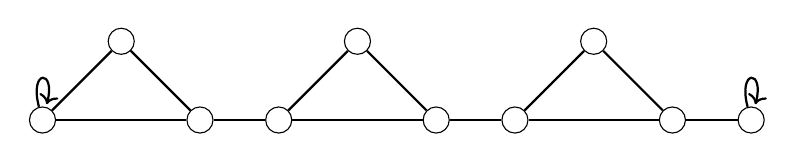
\begin{tikzpicture}[main node/.style={circle,draw}]

\node[main node] (n0) at (0,0) {};
\node[main node] (n1) at (1,1) {};
\node[main node] (n2) at (2,0) {};
\node[main node] (n3) at (3,0) {};
\node[main node] (n4) at (4,1) {};
\node[main node] (n5) at (5,0) {};
\node[main node] (n6) at (6,0) {};
\node[main node] (n7) at (7,1) {};
\node[main node] (n8) at (8,0) {};
\node[main node] (n9) at (9,0) {};

\path[] (n0) [-, thick, loop above] edge node [] {} (n0);
\path[] (n9) [thick, loop above] edge node [] {} (n9);
\path [] (n0) [-,thick] edge node [] {} (n1)
(n1) [-] edge node [] {} (n2)
(n0) [-] edge node [] {} (n2)
(n2) [-] edge node [] {} (n3)
(n3) [-] edge node [] {} (n4)
(n3) [-] edge node [] {} (n5)
(n4) [-] edge node [] {} (n5)
(n5) [-] edge node [] {} (n6)
(n6) [-] edge node [] {} (n7)
(n6) [-] edge node [] {} (n8)
(n7) [-] edge node [] {} (n8)
(n8) [-] edge node [] {} (n9);

\end{tikzpicture}
\end{center}

    \caption{Triangulated cycle distance. Notice that we went from $3$ vertices to $3(3)+1 = 10$ vertices.}
    \label{fig:graph15}
\end{figure}

Now that we have they are in the same cycle, we have that they will stay in the same cycle. We now focus on the lazy random walk on the triangulated cycle, with the addendum that on the vertices of degree $2$ (the top vertices of the triangles) we have a $2/3$ chance of staying in place. We'll couple so that they move to the top vertex together, move independent of one another on the bottom vertices (flip a coin and move either left or right), and otherwise move to opposite locations on the base from the top vertex. Using the same philosophy as with the normal cycle, we instead look at the Markov chain constructed by the clockwise distances between the vertices, with absorption at $0$ and $3n+1$ (here, $3n+1$ since there are now $3n$ vertices and we add an extra vertex to denote coalescing). An example of this can be seen in Figure \ref{fig:graph15}. 
\begin{claim}
Let $g_i$ be the expected value of being absorbed starting at the right most vertex in the $i$\textsuperscript{th} triangle, $h_i$ the left most vertex on the $i$\textsuperscript{th} triangle, and $f_i$ on the top most vertex on the $i+1$\textsuperscript{th} triangle. Then we have
\[ g_i = \frac{18+45(i-1)}{5} + \frac{5i-3}{5i} h_{i+1}.\]
\end{claim}
\begin{proof}
This can be shown using the usual inductive argument. In the case of $i=1$, we get 
\[g_1 = \frac{18}{5} + \frac{2}{5}h_2 \]
by simply substituting in the appropriate values. Assuming it holds for $i$, we simply need to substitute in appropriate values on this chain and we should get the result. So we have 
\[g_i = \frac{18 + 45(i-1)}{5} + \frac{5i-3}{5i}h_i, \]
\[ h_i = \frac{1}{6}(1+ g_i) + \frac{1}{6}(1+f_i) + \frac{1}{6}(1+g_{i+1}) + \frac{1}{2}(1+h_i),\]
and
\[ f_i = \frac{1}{6}(1+h_i) + \frac{1}{6}(1+g_{i+1}) + \frac{2}{3}(1+f_i). \]
Solving all of these variables and then solving for
\[g_{i+1} = \frac{1}{6}(1+h_i) + \frac{1}{6}(1+f_i) + \frac{1}{6}(1+g_{i+2}) + \frac{1}{2}(1+g_{i+1}) \]
gives us 
\[g_{i+1} = \frac{18 + 45i}{5} + \frac{5i+2}{5i+5}h_{i+1}. \]
as desired. 
\end{proof}
\begin{claim}
Letting $k = n/2$, we have
\[g_l = \frac{3}{5}(5k-5l+3)(5l-3). \]
\end{claim}

\begin{proof}
This holds for the base case $l = k$. Assume it holds for $i$. We must show it holds for $i-1$. Going through the motions, we have
\[f_i = \frac{1}{6}(1+g_i) + \frac{1}{6}(1+h_i) + \frac{2}{3}(1+f_i) \]
which solving gives us 
\[ f_i = \frac{3}{10}+\frac{15}{2}ki-\frac{9}{2}k-\frac{15}{2}{i}^{2}+9i+\frac{1}{2}h_i. \]
Solving 
\[h_i = \frac{1}{6}(1 + g_{i-1}) + \frac{1}{6}(1 + f_{i}) + \frac{1}{6}(1+g_i) + \frac{1}{2}h_i \]
gives us 
\[h_i = \frac{9}{25} + 9ki -\frac{27}{5}k - 9i^2 + \frac{54}{5}i + \frac{2}{5}g_{i-1}. \]
Finally, using the prior claim, we have
\[g_{i-1} = \frac{18+45\left((i-1)-1\right)}{5} + \frac{5(i-1)-3}{5(i-1)}h_i. \]
Substituting in the $h_i$ we just found, we get 
\[ g_{i-1} = -\frac{3}{5}(5i-5k-8)(5i-8), \]
which satisfies the induction hypothesis.
\end{proof}

This then also gives us 
\[h_l = 15(l-1)(k-l+1)\]
and
\[f_l =  -\frac{36}{5}+15\,kl-12\,k-15\,{l}^{2}+24l\]
for free by substitution. The top most node will be furthest away, so maximizing $f_l$ with respect to $l$ gives
\[ \frac{15}{16}n^2 + \frac{12}{5}. \]
Adding in the constant of $21$ we found earlier gives us 
\[ \max_{x,y \in \Omega} \mathbf{E}(\tau \ | \ X_0 = x, Y_0 =y) \leq \frac{15}{16}n^2 + \frac{87}{5}. \]
\end{proof}


\begin{corollary}
For the modified lazy random walk on the triangulated M\"{o}bius ladder graph, we have that the mixing time is 
\[ t_{\text{mix}}(\epsilon) \leq \frac{15 n^2}{16 \epsilon} + {87}{5\epsilon}.\]
\end{corollary}

\begin{proof}
The argument is analogous to the argument found in Corollary ~\ref{cor:one}.
\end{proof}

We then can also explore another nice class of $3$-regular graphs called \textbf{generalized Petersen graphs}, denoted by $\text{GP}(n,k)$. 

\begin{definition}
The generalized Petersen graph is constructed by having a cycle graph of size $n$ on the outside connected to the star polygon of size $n$ with $k$ vertices between a vertex and its neighbor. Notice that we require $n \geq 3$ and $ 1 \leq k \leq \lfloor (n-1)/2 \rfloor$. Notationally, we have again that a graph $G = (V,E)$ is the generalized Petersen graph $G(n,k)$ if
\[ V = \{(a,b) \ | \ a \in \{0,1\}, b \in \{0, \ldots, n-1\} \},\]
\[ E = \{\left((a,b),(c,d)\right) \ | \ a \neq c, b = d \text{ or } \]
\[ a = c = 1, b = d \ \pm \ 1 \Mod{n} \text{ or } a = c = 0, b = d \ \pm \ k \Mod{n}  \}.  \]
\end{definition}

Prism graphs are an example of $GP(n,1)$ for example. Another example can be seen in Figure \ref{fig:graph13}. We can use a similar sort of coupling procedure as we used with the prism and M\"{o}bius graphs to find a bound for $\text{GP}(n,k)$.

\begin{figure}

    \begin{center}
        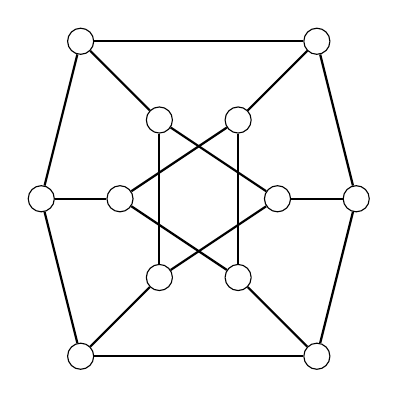
\begin{tikzpicture}[main node/.style={circle,draw}]

\node[main node] (n0) at (2,3) {};
\node[main node] (n1) at (3,3) {};
\node[main node] (n2) at (3.5,4) {};
\node[main node] (n3) at (3,5) {};
\node[main node] (n4) at (2,5) {};
\node[main node] (n5) at (1.5,4) {};
\node[main node] (n6) at (1,2) {};
\node[main node] (n7) at (4,2) {};
\node[main node] (n8) at (4.5,4) {};
\node[main node] (n9) at (4,6) {};
\node[main node] (n10) at (1,6) {};
\node[main node] (n11) at (0.5, 4) {};


\path[] (n6) [-,thick] edge node [] {} (n7);
\path[] (n7) [-,thick] edge node [] {} (n8);
\path[] (n8) [-,thick] edge node [] {} (n9);
\path[](n9) [-,thick] edge node [] {} (n10);
\path[](n10) [-,thick] edge node [] {} (n11);
\path[](n11) [-,thick] edge node [] {} (n6);

\path[](n0) [-,thick] edge node [] {} (n4);
\path[](n4) [-,thick] edge node [] {} (n2);
\path[](n2) [-,thick] edge node [] {} (n0);

\path[](n1) [-,thick] edge node [] {} (n3);
\path[](n3) [-,thick] edge node [] {} (n5);
\path[](n5) [-,thick] edge node [] {} (n1);


\path[](n0) [-,thick] edge node [] {} (n6);
\path[](n1) [-,thick] edge node [] {} (n7);
\path[](n2) [-,thick] edge node [] {} (n8);
\path[](n3) [-,thick] edge node [] {} (n9);
\path[](n4) [-,thick] edge node [] {} (n10);
\path[](n5) [-,thick] edge node [] {} (n11);
\end{tikzpicture}
\end{center}
    \caption{The generalized Petersen graph $\text{GP}(6,2).$}
    \label{fig:graph13}
\end{figure}

\begin{proposition}\label{prop:bb}
For the lazy random walk on $\text{GP}(n,k)$, we have that the mixing time is 
\[ t_{\text{mix}} \leq \frac{3 d^2}{2\epsilon}  + \frac{3}{2\epsilon} \bigg( \frac{n}{d}\bigg)^2 + \frac{18}{\epsilon},\]
where $d = n/\gcd (n,k)$.
\end{proposition}


\begin{figure}

    \begin{center}
    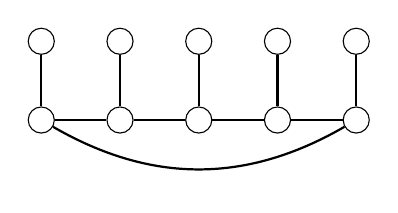
\begin{tikzpicture}[main node/.style={circle,draw}]

\node[main node] (n0) at (0,0) {};
\node[main node] (n1) at (0,1) {};
\node[main node] (n2) at (1,0) {};
\node[main node] (n3) at (1,1) {};
\node[main node] (n4) at (2,0) {};
\node[main node] (n5) at (2,1) {};
\node[main node] (n6) at (3,0) {};
\node[main node] (n7) at (3,1) {};
\node[main node] (n8) at (4,0) {};
\node[main node] (n9) at (4,1) {};

\path[] (n0) [-,thick] edge node [] {} (n1);
\path[] (n0) [-,thick] edge node [] {} (n2);
\path[] (n2) [-,thick] edge node [] {} (n3);
\path[] (n2) [-,thick] edge node [] {} (n4);
\path[] (n4) [-,thick] edge node [] {} (n5);
\path[] (n4) [-,thick] edge node [] {} (n6);
\path[] (n6) [-,thick] edge node [] {} (n7);
\path[] (n6) [-,thick] edge node [] {} (n8);
\path[] (n8) [-,thick] edge node [] {} (n9);
\path[] (n8) [-, bend left,thick] edge node [] {} (n0);

\end{tikzpicture}
\end{center}
    \caption{The cycle with extra nodes.}
    \label{fig:graph14}
    
\end{figure}

\begin{proof}

We first couple our walkers so that they have the same height; i.e., they are either on the inner cycles or on the outer cycle. Letting the walkers move independently of one another, we find that the probability of them coalescing with regards to inner or outer cycle, or height, is a geometric random variable with probability $1/6$. The expected value is then $6$. Once the walkers share the same height, they will always share the same height. The number of different cycles on the inner part is $d = n/\gcd (n,k)$, since we're looking at the order of $k$ in $\mathbb{Z}/n\mathbb{Z}$. We'll have our walkers move together on the inner part (so they move left, right, or outward together), and on the outer part they'll move independently of one another. Then we see that this gives us the quotient Markov chain on the cycle $n/d$ with extra nodes coming outward. An example of this can be seen in Figure \ref{fig:graph14}. We can use the same philosophy as on the normal cycle; shifting this to a Markov chain on $\{0, \ldots, n/d\}$ with absorbing $0$ and $n/d$ being absorbing states. Focusing only on the nodes on the `inside' portion, we set up a series of equations again.
\begin{claim}\label{claim:naya}
If $\tau$ is the amount of time it takes to be absorbed, letting $f_j = \mathbf{E}(\tau \ | \ X_0 = j)$, we have
\[ f_j = 6j + \frac{j}{j+1}f_{j+1},\]
$1 < j < n/d-1$.
\end{claim}

\begin{proof}
Notice that we have 
\[f_1 = \frac{1}{6}(1 + 0) + \frac{1}{6}(1+f_2) + \frac{1}{6}(1+g_1) + \frac{1}{2}(1+f_1), \]
where $g_i$ here denotes the outer nodes. For $g_i$, we have 
\[g_i = \frac{5}{6}(1+g_i) + \frac{1}{6}(1+f_i), \]
and solving this gives
\[g_i = 6 + f_i. \]
Substituting in all the values gives
\[f_1 = 6 + \frac{1}{2}f_2, \]
so we have Claim ~\ref{claim:naya} holds for the base case. Now, assume the inductive hypothesis holds for $j$. We show it holds for $j+1$. We set up 
\[f_{j+1} = \frac{1}{6}(1+f_j) + \frac{1}{6}(1+g_j) + \frac{1}{6}(1+f_{j+2}) + \frac{1}{2}(1+f_j). \]
Substituting in values and solving gives
\[f_{j+1} = 6(j+1) + \frac{j+1}{j+2}f_{j+2} \]
as desired.
\end{proof}

\begin{claim}\label{claim:grixis}
We have
\[f_j = 6j\bigg(\frac{n}{d}-j\bigg).\]
\end{claim}

\begin{proof}
From the prior claim, we have 
\[f_{n/d-1} = 6\left(\frac{n}{d}-1\right). \]
Assume Claim ~\ref{claim:grixis} holds by induction for $i$, and we want to show it holds for $i-1$. Then we have 
\[ f_i = 6i\left(\frac{n}{d}-i\right)\]
and
\[ f_{i-1} = 6(i-1) + \frac{i-1}{i} f_i.\]
Substituting in the values gives us 
\[f_{i-1} = 6(i-1)\left(\frac{n}{d}-i+1\right) \]
as desired.
\end{proof}

Maximizing this, and using the fact that $g_i > f_i$ for all $i$, we have an upper bound of $(3/2)(n/d)^2+6.$ Now that the walkers are in the same inner cycle (since there are $d$ inner cycles that we could possibly be in), we can couple with respect to the inner cycle, measuring how long it takes for the walkers to coalesce on their respective inner cycle. However, this is just the same process as in Claims \ref{claim:naya} and \ref{claim:grixis}, replacing $n/d$ with $d$. Once we have this, we sum everything together to see that 
\[d(t) \leq \frac{3}{2t}\bigg(\frac{n}{d}\bigg)^2 + \frac{3d^2}{2t} + \frac{18}{t}.\]
as desired.
\end{proof}

% ~639 in maple

\begin{proposition}\label{prop:sf}
For the lazy random walk on the triangulated $\text{GP}(n,k)$, we have that the mixing time is 
\[t_{\text{mix}} \leq \frac{15 d^2}{2\epsilon} + \frac{15}{2\epsilon} \bigg( \frac{n}{d}\bigg)^2 + \frac{9n}{d\epsilon} + \frac{9 d}{\epsilon} + \frac{96}{\epsilon}. \]
\end{proposition}

\begin{proof}


\begin{figure}

    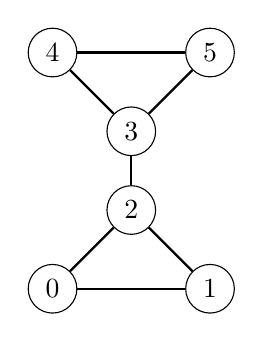
\begin{tikzpicture}[main node/.style={circle,draw}]
  
  \node[main node] (n0) at (0,0) {0};
  \node[main node] (n1) at (2,0) {1};
  \node[main node] (n2) at (1,1) {2};
  \node[main node] (n3) at (1,2) {3};
  \node[main node] (n4) at (0,3) {4};
  \node[main node] (n5) at (2,3) {5};
 \path[]
 (n0) [-,thick] edge node [] {} (n1)
 (n0) [-] edge node [] {} (n2)
 (n2) [-] edge node [] {} (n1)
 (n2) [-] edge node [] {} (n3)
 (n3) [-] edge node [] {} (n4)
 (n4) [-] edge node [] {} (n5)
 (n3) [-] edge node [] {} (n5);
 
\end{tikzpicture}
    \caption{Triangles in the Cycle}
    \label{fig:graph12}
\end{figure}

We will walk through roughly the same steps as before. We first couple our walkers so they are in the same position in their relative triangle. Moving our walkers independently, this is a geometric random variable and so it takes on average $6$ steps. We then want to couple our walkers so that they are in the same `height' on their respective triangle duo. See Figure \ref{fig:graph12} for an example. We couple so that if our walkers move to the top of their respective triangles ($2$ or $3$ in Figure \ref{fig:graph12}), then they move together. Once they are at the top of their triangles, then they coalesce with probability $1/3$ (one hops and the other stays in place), stay with probability $1/3$, and move downward with probability $1/3$. and once they are coupled in height then they stay coupled in height. Setting up a series of recursive functions, we find that this is bounded by $15$. Once coupled with regards to height, we then want to couple based on which inner cycle we are in, as in the proof of Proposition 12.

This gives us a cycle of length $n/d$ of triangles with triangles above it as well. An example of what each state looks like can be seen in Figure \ref{fig:graph12} again. We then would like to find the maximum expected amount of time it takes to coalesce on the cycle. Let the walkers move together everywhere except for the base of the triangle and left and right independently on the base of the triangle (that is, one stays in place while the other moves left or right). When moving downward from the top vertex of the base triangle, the walkers move to opposing spaces. We can then preform a similar procedure as in the proof of Proposition 11, with now the maximum expected time being at either of the top two vertices. 

\begin{claim}\label{claim:twen}
Take $f_i$ to be the far right vertex on the base of the $i$\textsuperscript{th} triangle (for example, $1$ in Figure \ref{fig:graph12}) and $h_{i}$ the left vertex on the base of the $i$\textsuperscript{th} triangle. Then we have
\[f_i = 18i + \frac{8+5(i-1)-3}{8+5(i-1)}h_{i+1}. \]
\end{claim}

\begin{proof}
We proceed by induction. For the base case, we just plug in values to get 
\[f_1 = 18 + \frac{5}{8}h_2. \]
Let $k_i$ be the vertex above $h_i$ and $f_i$ (for example, $2$ in Figure \ref{fig:graph12}), $a_i$ be the vertex above that (for example, see $3$ in Figure \ref{fig:graph12}), $d_i$ and $g_i$ the vertices on the top left and right respectively (for example, see $4$ and $5$ respectively in Figure \ref{fig:graph12}). Now, we assume Claim \ref{claim:twen} holds for $i$ and show it holds for $i+1$. Using our series of equation, we have 
\[f_i = 18i + \frac{8+5(i-1)-3}{8+5(i-1)}h_{i+1}, \]
\[h_{i+1} = \frac{1}{6}(1+f_{i+1}) + \frac{1}{6}(1+f_i) + \frac{1}{6}(1+k_{i+1}) + \frac{1}{2}(1+h_{i+1}), \]
\[k_{i+1} = \frac{1}{6}(1 + h_{i+1}) + \frac{1}{6}(1+f_{i+1}) + \frac{1}{6}(1+a_{i+1}) + \frac{1}{2}(1+k_{i+1}), \]
\[a_{i+1} = \frac{1}{6}(1+k_{i+1}) + \frac{1}{6}(1+d_{i+1}) + \frac{1}{6}(1+g_{i+1}) + \frac{1}{2}(1+a_{i+1}), \]
\[d_{i+1} = \frac{1}{6}(1+a_{i+1}) + \frac{1}{3}(1+g_{i+1}) + \frac{1}{2}(1+d_{i+1}), \]
\[g_{i+1} = \frac{1}{6}(1+a_{i+1}) + \frac{1}{3}(1+d_{i+1}) + \frac{1}{2}(1+g_{i+1}), \]
\[f_{i+1} = \frac{1}{6}(1+h_{i+1}) + \frac{1}{6}(1+k_{i+1}) + \frac{1}{6}(1+h_{i+2}) + \frac{1}{2}(1+f_{i+1}). \]
Solving and substituting in values gives us 
\[f_{i+1} = 18(i+1) + \frac{5+5i}{8+5i} h_{i+2} \]
as desired.
\end{proof}

\begin{claim}\label{claim:ninet}
Without loss of generality, take $g_i$ be the top right vertex of the $i$\textsuperscript{th} triangle (for example, $5$ in Figure \ref{fig:graph12}), and take $f_i$ to be the far right vertex on the base (for example, $1$ in Figure \ref{fig:graph12}). Then we have
\[g_i = \frac{198 + 30(i-1)}{5} + \frac{5i-1}{5i}f_{i}. \]
\end{claim}

\begin{proof}
Manually going through, we see we have
\[g_1 = \frac{198}{5} + \frac{4}{5}f_1. \]
Using the proof from the prior claim, we see that 
\[g_{i+1} = \frac{198+30(i)}{5} + \frac{5(i+1)-1}{5(i+1)}f_{i+1} \]
as desired. 
\end{proof}

\begin{claim}\label{claim:twenty}
We have
\[f_i = 6i \Bigg(5 \bigg(\frac{n}{d}\bigg) - 5i + 3\Bigg). \]
\end{claim}

\begin{proof}
Let $\alpha = n/d = \gcd(n,d)$ for notational simplicity. We have $h_{\alpha+1} = 0$, and so it follows that $f_{\alpha} = 18\alpha$, as desired from Claim \ref{claim:twen}. Now we check it holds for induction. Assume it holds for $i+1$, then we want to show it holds for $i$. Then using the values we found from the proof of Claim \ref{claim:twen}, we substitute in
\[f_{i+1} = 6(i+1) \left( 5\alpha - 5(i+1) + 3\right) \]
and we see that
\[f_i = 6i(5 \alpha-5i+3) \]
as desired.   
\end{proof}

\begin{claim}
We have
\[g_i = -30{i}^{2}+ \left( 30 \alpha +30 \right) i-6 \alpha +30 \]
\end{claim}

\begin{proof}
A consequence of Claims ~\ref{claim:ninet} and ~\ref{claim:twenty}.
\end{proof}

\noindent Maximizing $g_i$ with respect to this gives us
\[\max_{x,y \in \Omega} \mathbf{E}(\tau \ | \ X_0 = x, Y_0 =y) \leq \frac{15}{2} \bigg(\frac{n}{d}\bigg)^2 + 9 \frac{n}{d} + \frac{75}{2}. \]
As in Proposition 12, we repeat this process for the inner triangles, with coalescing here now meaning our walkers coalesce in the larger triangle. Repeating this procedure now gives 
\[\max_{x,y \in \Omega} \mathbf{E}(\tau \ | \ X_0 = x, Y_0 =y) \leq \frac{15}{2} d^2 + 9 d^2 + \frac{75}{2}. \]
We then sum these together along with our constant value to get our result.
\end{proof}

In the prism graph, M\"{o}bius ladder graph, and generalized Petersen graph, we see that (fixing $k$) the triangulated version is asymptotically $5$ times larger than the non-triangulated version of the graph. This then leads us to a few questions.

\begin{question}\label{question:one}
For vertex transitive $3$-regular graphs, is the mixing time of the triangulated $3$-regular graph at most asymptotically $5$ times larger than the upper bound of the mixing time of the non-triangulated version?
\end{question}

\begin{question}
For all $3$-regular graphs, is the mixing time of the triangulated $3$-regular graph always asymptotically $5$ times larger than the upper bound of the mixing time of the non-triangulated version?
\end{question}

\begin{question}
Can we find similar results for the lower bounds on these mixing times?
\end{question}

\begin{question}
Are these bounds tight?
\end{question}


Further research on this could explore these questions. Propositions \ref{prop:funsies}, \ref{prop:stup}, \ref{prop:bb}, and \ref{prop:sf} all give some evidence towards Question 4.1. Being able to classify graphs like the Heawood and Franklin graph may provide further evidence or counterexamples for Question 4.1. For Questions 4.2 and 4.3, one may want to explore $3$-regular graphs with large bottlenecks. It seems like vertex transitivity is a required property for this to work based on how the couplings in the prior examples worked, so explicitly finding a family of $3$-regular graphs which are not vertex transitive and determining the asymptotics of the mixing time for the non-triangulated and triangulated version may provide counter examples for Question 4.2. Finally, methods other than coupling may shed some light on Question 4.4.

\section{Appendix}\label{appendix}

Throughout, we mention things like Gambler's ruin and the mixing time on the cycle of length $n$. While these facts can be found in most textbooks on Markov chains and mixing times (see \cite{durrett1999essentials},\cite{LevinPeresWilmer2006}, \cite{resnick2013adventures}), we place them here for convenience.

\begin{proposition}[Fair Gambler's Ruin] \label{prop:gambleruin}
If a Gambler is betting $1$ dollar on flips of a fair coin, and must leave the game if they run out of money or reach $n$ dollars, then we have 
\[\mathbf{E}(\tau \ | \ X_0 = k) = k(n-k), \]
where $\tau$ is the amount of time it takes to reach $0$ or $n$.
\end{proposition}

\begin{proof}
Let $f_i = \mathbf{E}(\tau \ | \ X_0 = i)$. Then we have $f_0 = 0 = f_n$, and 
\[f_i = \frac{1}{2}(1+f_{i-1}) + \frac{1}{2}(1+f_{i+1}). \]
This leads us to the following claim.
\begin{claim}
We have 
\[ f_i = i + \frac{i}{i+1} f_{i+1}\]
for $0 < i < n$.
\end{claim}

\begin{proof}
We proceed by induction. For the base case, we have 
\[f_1 = \frac{1}{2}(1+0) + \frac{1}{2}(1+f_2) \]
and so simplifying gives us 
\[f_1 = 1 + \frac{1}{2} f_2. \]
Assume it holds for $i$. Then we have
\[ f_{i+1} = \frac{1}{2}(1+f_i) + \frac{1}{2}(1+f_{i+2}).\]
Substituting in $f_i$ and solving for $f_{i+1}$ gives
\[f_{i+1} = i+1 + \frac{i+1}{i+2}f_{i+2} \]
as desired.
\end{proof}

We now need to establish the claim by induction. For the base case, we have
\[f_{n-1} = n-1 + \frac{n-1}{n} (0) = n-1 = (n-1)\big(n-(n-1)\big). \]
Assume it holds for $k$; that is,
\[f_k = k(n-k). \] 
Then we have
\[f_{k-1} = k-1 + \frac{k-1}{k} f_k. \]
By the prior claim, we get 
\[f_{k-1} = k-1 + \frac{k-1}{k} \big(k(n-k)\big) = k-1 + (n-k)(k-1)\]
\[= \big(1+(n-k)\big)(k-1) = (k-1)\big(n-(k-1)\big) \]
as desired. So the inductive hypothesis holds, and we get 
\[ f_k = k(n-k)\]
for all $0 < k < n$ as desired. In particular, maximizing this gives 
\[\max_{x,y \in \Omega} \mathbf{E}(\tau \ | \ X_0 = x, Y_0 = y) \leq \frac{n^2}{4}.\]
\end{proof}

\begin{proposition}[Mixing Time of the Cycle]
We have that the mixing time on the cycle $\mathbb{Z}/n\mathbb{Z}$ is bounded above by
\[ t_{\text{mix}}(\epsilon) \leq \frac{n^2}{4\epsilon}.\]
\end{proposition}

\begin{proof}
Our coupling procedure is as follows: flip a fair coin to determine which walker we move. Then, flip another fair coin to determine whether the walker moves left or right. We measure the clockwise distance between the two walkers after each step. The coupling procedure then shifts us to a walk on the chain $\{0 \ldots, n\}$, with $0$ and $n$ being absorbing states and transition probabilities being $1/2$. We can then use Proposition \ref{prop:gambleruin} to determine that 
\[ \max_{x,y \in \Omega} \mathbf{E}(\tau \ | \ X_0 = x, Y_0 =y) \leq \frac{n^2}{4}, \]
and so using Theorem \ref{thm:2} we get 
\[t_{\text{mix}} \leq \frac{n^2}{4\epsilon}. \]
\end{proof}

\bibliography{citations}
\bibliographystyle{plain}

\end{document}
